\documentclass{pluto}




 
\title{\bf Java学习笔记}                                                      % Supply information
\author{白水}                                                                % for the title page.
\date{\today}                                                               % Use current date. 

\begin{document}
\begin{titlepage}
    \begin{center}
        \vspace*{1cm}
        \Huge
        \textbf{学习笔记}
        \vspace{0.5cm}

        \vfill
        \large
            \textit{Java}
            \vfill
   
            \vfill
            
\includegraphics[width=0.1\textwidth]{logo.png}
    \end{center}
\end{titlepage}

\frontmatter                                                                % End of preamble, start of text.

\tableofcontents

\mainmatter

\part{Java基础知识}
\chapter{JVM}
\label{chap:jvm}




\chapter{基本语法}
\label{chap:grammar}


\section{基本规范}

\textbf{Java区分大小写}

Java采用骆驼命名法,CamelCase。

\section{数据类型}

Java包含8种基本类型。\par
\begin{itemize}
        \item   4种整型
        \item   2种浮点类型 
        \item   1种表示Unicode编码的字符单元的字符类型char
        \item   1种表示真值的boolean类型
\end{itemize}


\subsection{整型}

\renewcommand\arraystretch{2}
\begin{tabular}{l|l|l}
    类型        &      存储需求        &     取值范围        \\               \hline
    byte       &       1字节          & -128 $\sim$ 127     \\
    short      &       2字节          & -32768 $\sim$ 32767  \\
    int        &       4字节          &  -2147483648 $\sim$ 2147483647  \\
    long       &       8字节          &  -9223372036854775808 $\sim$ 9223372036854775807  \\
\end{tabular}\newline

\notebox{Java 没有任何无符号(unsigned)形式的整型。}

长整型值有一个后缀l或者L。

\begin{lstlisting}[style=cjava]
        long number = 123L;             // number值为:123
\end{lstlisting}


\begin{itemize}
    \item   二进制带前缀0b或者0B (从java 7开始)
    \item   八进制带前缀0
    \item   十六进制带前缀0x或者0X
\end{itemize}


\begin{lstlisting}[style=cjava]
        int binaryNumber      = 0B101;              // 二进制表示   5 

        int hexadecimalNumber = 0x123;              // 十六进制表示 291   

        int octonaryNumber    = 0123;              // 八进制表示   83
\end{lstlisting}



同样从Java7开始为数字加下划线,Java编译器会去除这些下划线

\begin{lstlisting}[language=java]
        Sytem.out.println(0_1_0);       // 010表示八进制,输出8
\end{lstlisting}


toBinaryString


\cautionbox{
注意JS INT类型的值范围:
\begin{itemize}
        \item   \href{http://speakingjs.com/es5/ch11.html}{Integers in JavaScript} 
        \item   \href{http://speakingjs.com/es5/ch11.html\#safe\_integers}{Safe Integers}
        \end{itemize}
}


\subsection{浮点数}


\renewcommand\arraystretch{2}
\begin{tabular}{l|l|l}
    类型         &      存储需求        &     取值范围        \\               \hline
    float        &       4字节          & 有效位数为6-7位      \\
    double      &       8字节          & 有效位数为15位       \\
\end{tabular}\newline


float类型的值要有后缀f或者F。没有后缀默认为double类型。

double类型也可以添加d或者D后缀。


用于表示溢出或者出错情况的三个特殊浮点值:

\begin{itemize}
        \item   正无穷大  
        \item   负无穷大
        \item   NaN (不是一个数字)
\end{itemize}

例如: 一个正整数除以 0 的结果为正无穷大; 计算 0/0或者负数的平方根结果为NaN。

对应常量为:
\begin{lstlisting}[language=java]
        // float
        Float.POSITIVE_INFINITY;
        Float.NEGATIVE_INFINITY;
        Float.NaN;
        // double
        Double.POSITIVE_INFINITY;
        Double.NEGATIVE_INFINITY;
        Double.NaN;
\end{lstlisting}


所有“非数值”的值都认为是不相同的。

\begin{lstlisting}[language=java]
        if(Double.isNaN(x))   // check whether x is "not a number"
\end{lstlisting}




\textbf{char类型}


\section{运算符}

\subsection{位运算符}

\renewcommand\arraystretch{2}
\begin{tabular}{l|l|l}
    操作符    &     名称          &     说明                                                   \\   \hline
    \~{}     &  Not(按位取反)   & 一元运算符   \quad 0变为1、将1变为0                            \\
    \&       &   And(按位与)    & 二元运算符 \quad 两值全为1则为1 \quad 例:1\&1=1                \\
    |       &   Or(按位或)     & 二元运算符 \quad 两值有1则为1 \quad 例: 0|1=1                  \\
    \^{}     &   Xor(按位异或)  & 二元运算符 \quad 两值不相同则异或结果为1 \quad 例: 1\^{}0=1      \\
    <<       &  左移位           & 二元运算符 \quad                                              \\
    >>       &  右移位           & 二元运算符 \quad 符号运算符会填充高位                                \\ 
    >>>      & 无符号右移位       & 二元运算符 \quad 运算符会用0填充高位                             \\
\end{tabular}\newline


\textbf{移位}


字节顺序


对于w位的操作数$x$用位表示为 [$x_{w-1}$, $x_{w-2}$, ... , $x_{0}$, $x_{0}$ ]。
其中$x_{w-1}$是最高有效位,而$x_{0}$是最低有效位。

小端法(little endian): 选择在内存中按照从最低有效字节到最高有效字节的顺序存储对象

大端法(big endian): 选择在内存中按照从最高有效字节到最低字节的顺序存储对象

假设变量x的类型为int,位于地址0x100处,它的十六进制值为0x1234567。地址范围0x100 ~ 0x103的字节顺序。


\begin{figure}[H]
        \centering
        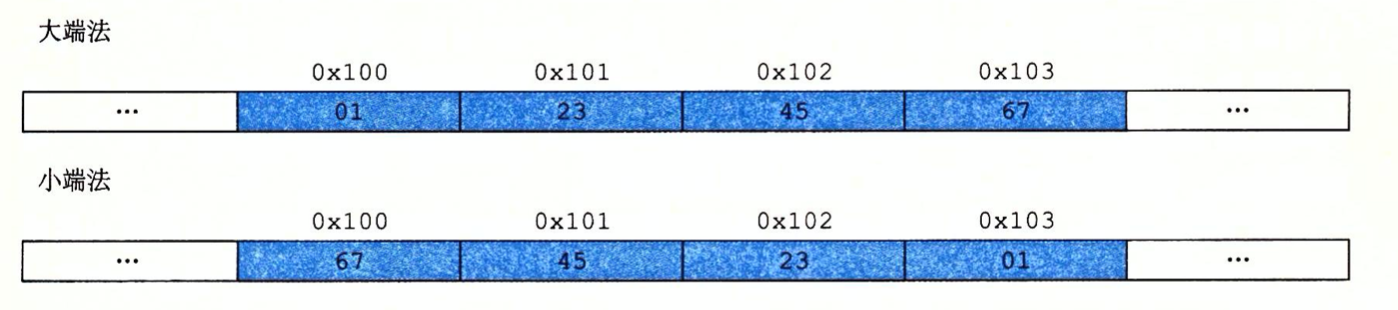
\includegraphics[width=1\textwidth]{basic/big_little_endian.png}
    \end{figure}


移位运算符的右操作数会先完成取模运算。int类型模32,long类型模64。


\begin{lstlisting}[language=java]

\end{lstlisting}




避免时序攻击的字符串比较

\begin{lstlisting}[language=java]

        static boolean equals(byte[] s1, byte[] s2) {
                if (s1.length != s2.length) {
                  return false;
                }
                char c = 0;
                for (int i = 0; i < s1.length; i++) {
                  c |= (s1[i] ^ s2[i]);
                }
                return c == 0;
              }
        
\end{lstlisting}














































\chapter{控制流程}
\label{chap:control_flow}

\section{switch}

\textbf{Java}

只支持基本类型(byte,short,char,int)、Enum类型以及String, Character, Byte, Short和Integer类。

只支持常量表达式,case会进行整数范围验证。

\begin{lstlisting}[style=cjava,caption={swtich},label=useless]
    /*
    * 枚举类型
    */
    public enum Day {
        SUNDAY, MONDAY, TUESDAY, WEDNESDAY,
        THURSDAY, FRIDAY, SATURDAY 
    }

    /*
    * 星期判断
    * @param day
    */
    public static void switchTestWithEnum(Day day) {
    switch (day) {
        case MONDAY:
            System.out.println("Today is Mondays.");
            break;
        default:
            System.out.println("Today is ...");
            break;
        }
   }

    public static void switchTestWithCharacter(Character character) {
        switch (character) {
            case 'a':
                System.out.println("character is a");
                break;
            case 'b':
                System.out.println("character is b");
            default:
                System.out.println("nothing...");
        }
    }

    //调用
    switchTestWithEnum(Day.SUNDAY);
    switchTestWithCharacter(new Character('a'));
\end{lstlisting}


\textbf{PHP}

case 表达式可以是任何求值为简单类型的表达式,即整型或浮点数以及字符串。不能用数组或对象,除非它们被解除引用成为简单类型。

允许使用分号代替 case 语句后的冒号

case比较执行的是松散比较 ==

 \begin{lstlisting}[language=php,caption={php-swtich},label=useless]
    $beer = 'caseC';
    $a ='caseA';

    switch($beer)
    {
	    case $a;
		    echo "this is caseA";
		break;
	    case 'caseB';
		    echo "this is caseB";
		break;
	    case 'case'.'C':
	        echo "this is caseC";
	    break;
        default;
            echo 'Please make a new selection...';
        break;
    }
\end{lstlisting}
    

\chapter{字符串}
\label{chap:string}

    Strings are constant; their values cannot be changed after they are created.

\section{字符串对象}

String对象是不可改变的,具有恒定性。

每个String对象都有常量值。

字符串字面常量是对String类的示例的饮用。

在Java中String对象可以认为是char数组的延伸和进一步的封装。

\begin{noteblock}
    这里所说的char数组不是C语言意义上的字符型数组,而是大致类似于C语言中的 char* 指针。 \par
    \begin{lstlisting}[style=cjava]
    String str = "Java学习笔记"; 
    \end{lstlisting}
    \begin{lstlisting}[style=cjava]
    char* str = "Java学习笔记";
    \end{lstlisting}
\end{noteblock}

\begin{lstlisting}[style=cjava]

    public final class String implements java.io.Serializable, Comparable<String>, CharSequence {

    /** The value is used for character storage. */
    private final char value[];

    /*
    * @param  value             Array that is the source of characters
    * @param  offset            The initial offset
    * @param  count             The length
    *
    * @throws  IndexOutOfBoundsException
    *          If the {@code offset} and {@code count} arguments index
    *          characters outside the bounds of the {@code value} array
    */
    public String(char value[], int offset, int count) {
        if (offset < 0) {
            throw new StringIndexOutOfBoundsException(offset);
        }
        if (count <= 0) {
            if (count < 0) {
                throw new StringIndexOutOfBoundsException(count);
            }
            if (offset <= value.length) {
                this.value = "".value;
                return;
            }
        }
        // Note: offset or count might be near -1>>>1.
        if (offset > value.length - count) {
            throw new StringIndexOutOfBoundsException(offset + count);
        }
        this.value = Arrays.copyOfRange(value, offset, offset+count);
    }

    }

\end{lstlisting}

通过上面String类的实现代码可以发现String类和value数组都是final类型,这就保证了String对象的不变性。这种不变性可以带来极大的好处。

\begin{itemize}
    \item 保证对String对象的任意操作都不会改变原字符串
    \item 意味着操作字符串不会出现线程同步问题
    \item 成就了字符串驻留以及共享(常量池)
\end{itemize}



\section{字符串连接操作符 + }


如果字符串连接操作符运算的结果不是编译时的常量表达式,那么该操作符会隐式地创建新的String对象。


如果只有一个操作数表达式是String 类型,那么就会在另一个操作数上执行字符串转换以在运行时产生字符串。 
对于简单类型Java还可以通过直接将简单类型转换为字符串而优化掉包装器对象的创建。

\textcolor{codepurple}{+}操作字符在语法上是左结合。

例如:

\begin{lstlisting}[style=cjava]

    String first = 1 + 2 + "Java";
    String second = "Java" + 1 + 2;
    String three = "Java" + null;
    System.out.println(first);
    System.out.println(second);
    System.out.println(three);

    /** 
    * Output: 
    * 
    * 3Java
    * Java12
    * Javanull
    * 
    */

\end{lstlisting}


在字符串转换方面要特别注意引用类型转行。

如果该引用是null,那么它转换为字符串"null"。

如果其他引用类型,则调用其对象上的toString()方法;如果调用toString()方法的结果是null,那么就用字符串"null"代替。


\section{字符串常量池}




\section{StringBuilder}









https://tech.meituan.com/2014/03/06/in-depth-understanding-string-intern.html

















































\chapter{内部类}
\label{chap:inner_class}

可以将一个类的定义放在另一个类的定义内部,这就是内部类。

内部类的对象与制造它的外围对象(enclosing object)之间就有一种联系,它能访问其外围对象的所有成员,而不要任何特殊条件。
内部类还拥有其外围类的所有元素的访问权。


\section{.this和.new}




Anonymous Inner Class

It is an inner class without a name and for which only a single object is created.
An anonymous inner class can be useful when making an instance of an object with certain “extras” such as overloading methods of a class or interface, without having to actually subclass a class.


are mainly created in two ways:

. Class (abstract or concrete)
. interface

The syntax of an anonymous class expression is like the invocation of a constructor, except that there is a class definition contained in a block of code.
匿名类表达式的语法类似于调用构造函数,只是在代码块中包含了一个类定义。

匿名内部类的创建格式

\begin{lstlisting}[style=cjava]
    new class(arguments) | interface()
    {
        //匿名内部类的类体部分
    }
\end{lstlisting}

okHttp中匿名类示例

\begin{lstlisting}[style=cjava]
    public abstract class Internal {
        public abstract void addLenient(Headers.Builder builder, String line);
    }

    Internal.instance = new Internal() {
        @Override public void addLenient(Headers.Builder builder, String line) {
        builder.addLenient(line);
        }
    }
\end{lstlisting}


Difference between Normal/Regular class and Anonymous Inner class:

A normal class can implement any number of interfaces but anonymous inner class can implement only one interface at a time.
A regular class can extend a class and implement any number of interface simultaneously. But anonymous Inner class can extend a class or can implement an interface but not both at a time.
For regular/normal class, we can write any number of constructors but we cant write any constructor for anonymous Inner class because anonymous class does not have any name and while defining constructor class name and constructor name must be same.


\subsection{嵌套类}

将内部类声明为static,内部类对象与其外围类对象之间则没有联系。

1. 要创建嵌套类的对象,并不需要其外围类的对象。
2. 不能从嵌套类的对象中访问非静态的外围类对象。




\chapter{对象}

\label{chap:object}

\section{初始化}


静态初始化只有在对象被创建或者第一次访问静态数据时才会被初始化。

初始化的顺序时先静态对象(如果他们尚未因前面的对象创建过程而被初始化),而后才是“非静态”对象。

以Dog类为示例总结一下对象的创建过程:

1. 当首次创建类型为Dog的对象或者Dog类的静态方法/静态域首次被访问时,java解释器必须查找类路径,以定位Dog.class文件

2.然后载入Dog.class ,有关静态初始化的所有动作都会执行。因此,静态初始化只在Class对象首次加载的时候进行一次。按照顺序。

3. 当用new Dog() 创建对象的时候,首先将在堆上为Dog对象分配足够的存储空间。

4. 这块存储空间会被清零,这就自动将Dog对象中的所有基本类型数据都设置成了默认值(数字为0,boolean为false),而引用则被设置成null(例如String)

5. 执行所有出现于字段定义处的初始化动作

6. 执行构造器(会涉及到继承的问题)


总结


基类静态代码块、基类静态成员字段并列优先级,按照代码中出现先后顺序执行(只有第一次加载类时执行)

派生类静态代码块、派生类静态成员字段并列优先级,按照代码中出现先后顺序执行(只有第一次加载类时执行)

基类普通代码块、基类普通成员字段并列优先级,按照代码中出现先后顺序执行

基类构造函数

派生类普通代码块、派生类普通成员字段并列优先级,按照代码中出现顺序执行

派生类构造函数

\subsection{对象拷贝}

对象的拷贝分为 shallow copy 和 deep copy 。

shallow copy 既浅拷贝。




https://zhuanlan.zhihu.com/p/26964202

\href{https://zgxxx.github.io/2019/02/27/20190227/}{clone}

\href{https://howtodoinjava.com/java/cloning/a-guide-to-object-cloning-in-java/}{clone}

PHP与Java一样,对象的对象属性都只是引用拷贝.

php的拷贝是通过clone关键字实现。






static

在static方法的内部不允许调用非静态方法,可以在没有创建任何对象的前提下,仅仅通过类本身来调用static方法。


初始化

初始化顺序

在类的内部,变量定义的先后顺序决定了初始化的顺序。

变量的初始化会在任何方法(包括构造器)被调用前得到初始化。



\chapter{范型}

\label{chap:generics}

\section{基本概念}

范型实现了参数化类型的概念。

\section{范型类}


\section{范型方法}

\section{通配符类型}

函数式接口

关于函数式接口

如果一个接口只有一个抽象方法,那么该接口就是一个函数式接口

如果我们在某个接口上声明了FunctionalInterface注解,那么编译器就会按照函数式接口的定义来要求该接口

如果某个接口只有一个抽象方法,但我们并没有给该接口声明FunctionalInterface注解,那么编译器依旧会将该接口看作是函数式接口

\begin{lstlisting}[style=cjava]
    List<Integer> list = Arrays.asList(1,2,3,4,5);

    list.forEach(new Consumer<Integer>(){
        @Override
        public void accept(Integer integer){
            System.out.println(integer);
        }
    });
\end{lstlisting}

在java中Lambda表达式是对象,他们必须依附与一类特别的对象类型-函数式接口(functional interface)

That instances of functional interfaces can be created with lambda expressions, method references, or constructor references.

函数式接口的实例可以通过lambda表达式,方法引用和构造函数引用创建。


外部迭代和内部迭代

Java lambda表达式是一种匿名函数;它是没有声明的方法,即没有访问修饰符,返回值声明和名字。

lambda操作符: ->
lambda左边:接口中抽象方法的形参列表
lamdba右边:重写抽象方法的方法体


当只有一个参数,并且类型可推导时,圆括号()可省略。例如: a-> return a*a

lambda 表达式的主体可包含零条或多条语句

如果lambda表达式的主体只有一条语句,花括号{} 可省略。匿名函数的返回类型与该主体表达式一致

如果Lambda表达式的主体包含一条以上语句,则表达式必须包含在花括号{}中。匿名函数的返回类型与代码块的返回类型一致,若没有返回值则为空



Function<T, R>
 
BiFunction<T, U, R>



\chapter{异常处理}

\section{异常}

\label{chap:exception}

异常的抛出同其他对象的创建一样,将使用new在堆上创建异常对象。然后当前的执行路径(它不能继续执行下去)被终止,并且从当前环境中弹出对异常对象的引用。
此时异常处理机制接管程序,并开始寻找一个恰当的地方来继续执行程序。而这个恰当的地方就是“异常处理程序”。它的任务是将程序从错误状态中恢复,以使程序能
要么换一种方式运行,要么继续运行下去。

Throwable类是所有异常的基类。

//此处有类图

Throwable Error Exception RuntimeException 非RuntimeException




\section{异常说明}

异常说明使用附加关键字throws。



重抛异常会把异常抛给上一级环境中的异常处理程序。同一个try块的后续catch子句将被忽略。




\begin{lstlisting}[language=java]
    
/**
 * The {@code Throwable} class is the superclass of all errors and
 * exceptions in the Java language. Only objects that are instances of this
 * class (or one of its subclasses) are thrown by the Java Virtual Machine or
 * can be thrown by the Java {@code throw} statement. Similarly, only
 * this class or one of its subclasses can be the argument type in a
 * {@code catch} clause.
 *
 * For the purposes of compile-time checking of exceptions, {@code
 * Throwable} and any subclass of {@code Throwable} that is not also a
 * subclass of either {@link RuntimeException} or {@link Error} are
 * regarded as checked exceptions.
 *
 * <p>Instances of two subclasses, {@link java.lang.Error} and
 * {@link java.lang.Exception}, are conventionally used to indicate
 * that exceptional situations have occurred. Typically, these instances
 * are freshly created in the context of the exceptional situation so
 * as to include relevant information (such as stack trace data).
 *
 * <p>A throwable contains a snapshot of the execution stack of its
 * thread at the time it was created. It can also contain a message
 * string that gives more information about the error. Over time, a
 * throwable can {@linkplain Throwable#addSuppressed suppress} other
 * throwables from being propagated.  Finally, the throwable can also
 * contain a <i>cause</i>: another throwable that caused this
 * throwable to be constructed.  The recording of this causal information
 * is referred to as the <i>chained exception</i> facility, as the
 * cause can, itself, have a cause, and so on, leading to a "chain" of
 * exceptions, each caused by another.
 *
 * <p>One reason that a throwable may have a cause is that the class that
 * throws it is built atop a lower layered abstraction, and an operation on
 * the upper layer fails due to a failure in the lower layer.  It would be bad
 * design to let the throwable thrown by the lower layer propagate outward, as
 * it is generally unrelated to the abstraction provided by the upper layer.
 * Further, doing so would tie the API of the upper layer to the details of
 * its implementation, assuming the lower layer's exception was a checked
 * exception.  Throwing a "wrapped exception" (i.e., an exception containing a
 * cause) allows the upper layer to communicate the details of the failure to
 * its caller without incurring either of these shortcomings.  It preserves
 * the flexibility to change the implementation of the upper layer without
 * changing its API (in particular, the set of exceptions thrown by its
 * methods).
 *
 * <p>A second reason that a throwable may have a cause is that the method
 * that throws it must conform to a general-purpose interface that does not
 * permit the method to throw the cause directly.  For example, suppose
 * a persistent collection conforms to the {@link java.util.Collection
 * Collection} interface, and that its persistence is implemented atop
 * {@code java.io}.  Suppose the internals of the {@code add} method
 * can throw an {@link java.io.IOException IOException}.  The implementation
 * can communicate the details of the {@code IOException} to its caller
 * while conforming to the {@code Collection} interface by wrapping the
 * {@code IOException} in an appropriate unchecked exception.  (The
 * specification for the persistent collection should indicate that it is
 * capable of throwing such exceptions.)
 *
 * <p>A cause can be associated with a throwable in two ways: via a
 * constructor that takes the cause as an argument, or via the
 * {@link #initCause(Throwable)} method.  New throwable classes that
 * wish to allow causes to be associated with them should provide constructors
 * that take a cause and delegate (perhaps indirectly) to one of the
 * {@code Throwable} constructors that takes a cause.
 *
 * Because the {@code initCause} method is public, it allows a cause to be
 * associated with any throwable, even a "legacy throwable" whose
 * implementation predates the addition of the exception chaining mechanism to
 * {@code Throwable}.
 *
 * <p>By convention, class {@code Throwable} and its subclasses have two
 * constructors, one that takes no arguments and one that takes a
 * {@code String} argument that can be used to produce a detail message.
 * Further, those subclasses that might likely have a cause associated with
 * them should have two more constructors, one that takes a
 * {@code Throwable} (the cause), and one that takes a
 * {@code String} (the detail message) and a {@code Throwable} (the
 * cause).
 *
 * @author  unascribed
 * @author  Josh Bloch (Added exception chaining and programmatic access to
 *          stack trace in 1.4.)
 * @jls 11.2 Compile-Time Checking of Exceptions
 * @since JDK1.0
 */

\end{lstlisting}




\section{异常捕获}

try.catch.finally

Java7开始,可以在一个catch表达式中对多种类型异常进行合并捕获。

\begin{lstlisting}[language=java]
    public int getBinaryInt(String number) {
        int result = -1;
        result = result / 2;
        try {
            result = Integer.parseInt(number, 2);
        } catch (NumberFormatException | ArithmeticException e) {
                
        }

        return result;
    }
\end{lstlisting}



\chapter{线程}
\label{chap:thread}

\section{线程基础知识}

\subsection{线程状态}

JVM线程的状态定义在Thread.State枚举中。包括:

\begin{itemize}
    \item   NEW         新建
    \item   RUNNABLE    就绪
    \item   BLOCKED     阻塞 
    \item   WAITING     
    \item   TIMED\_WAITING
    \item   TERMINATED
\end{itemize}


\begin{figure}[H]
    \centering
    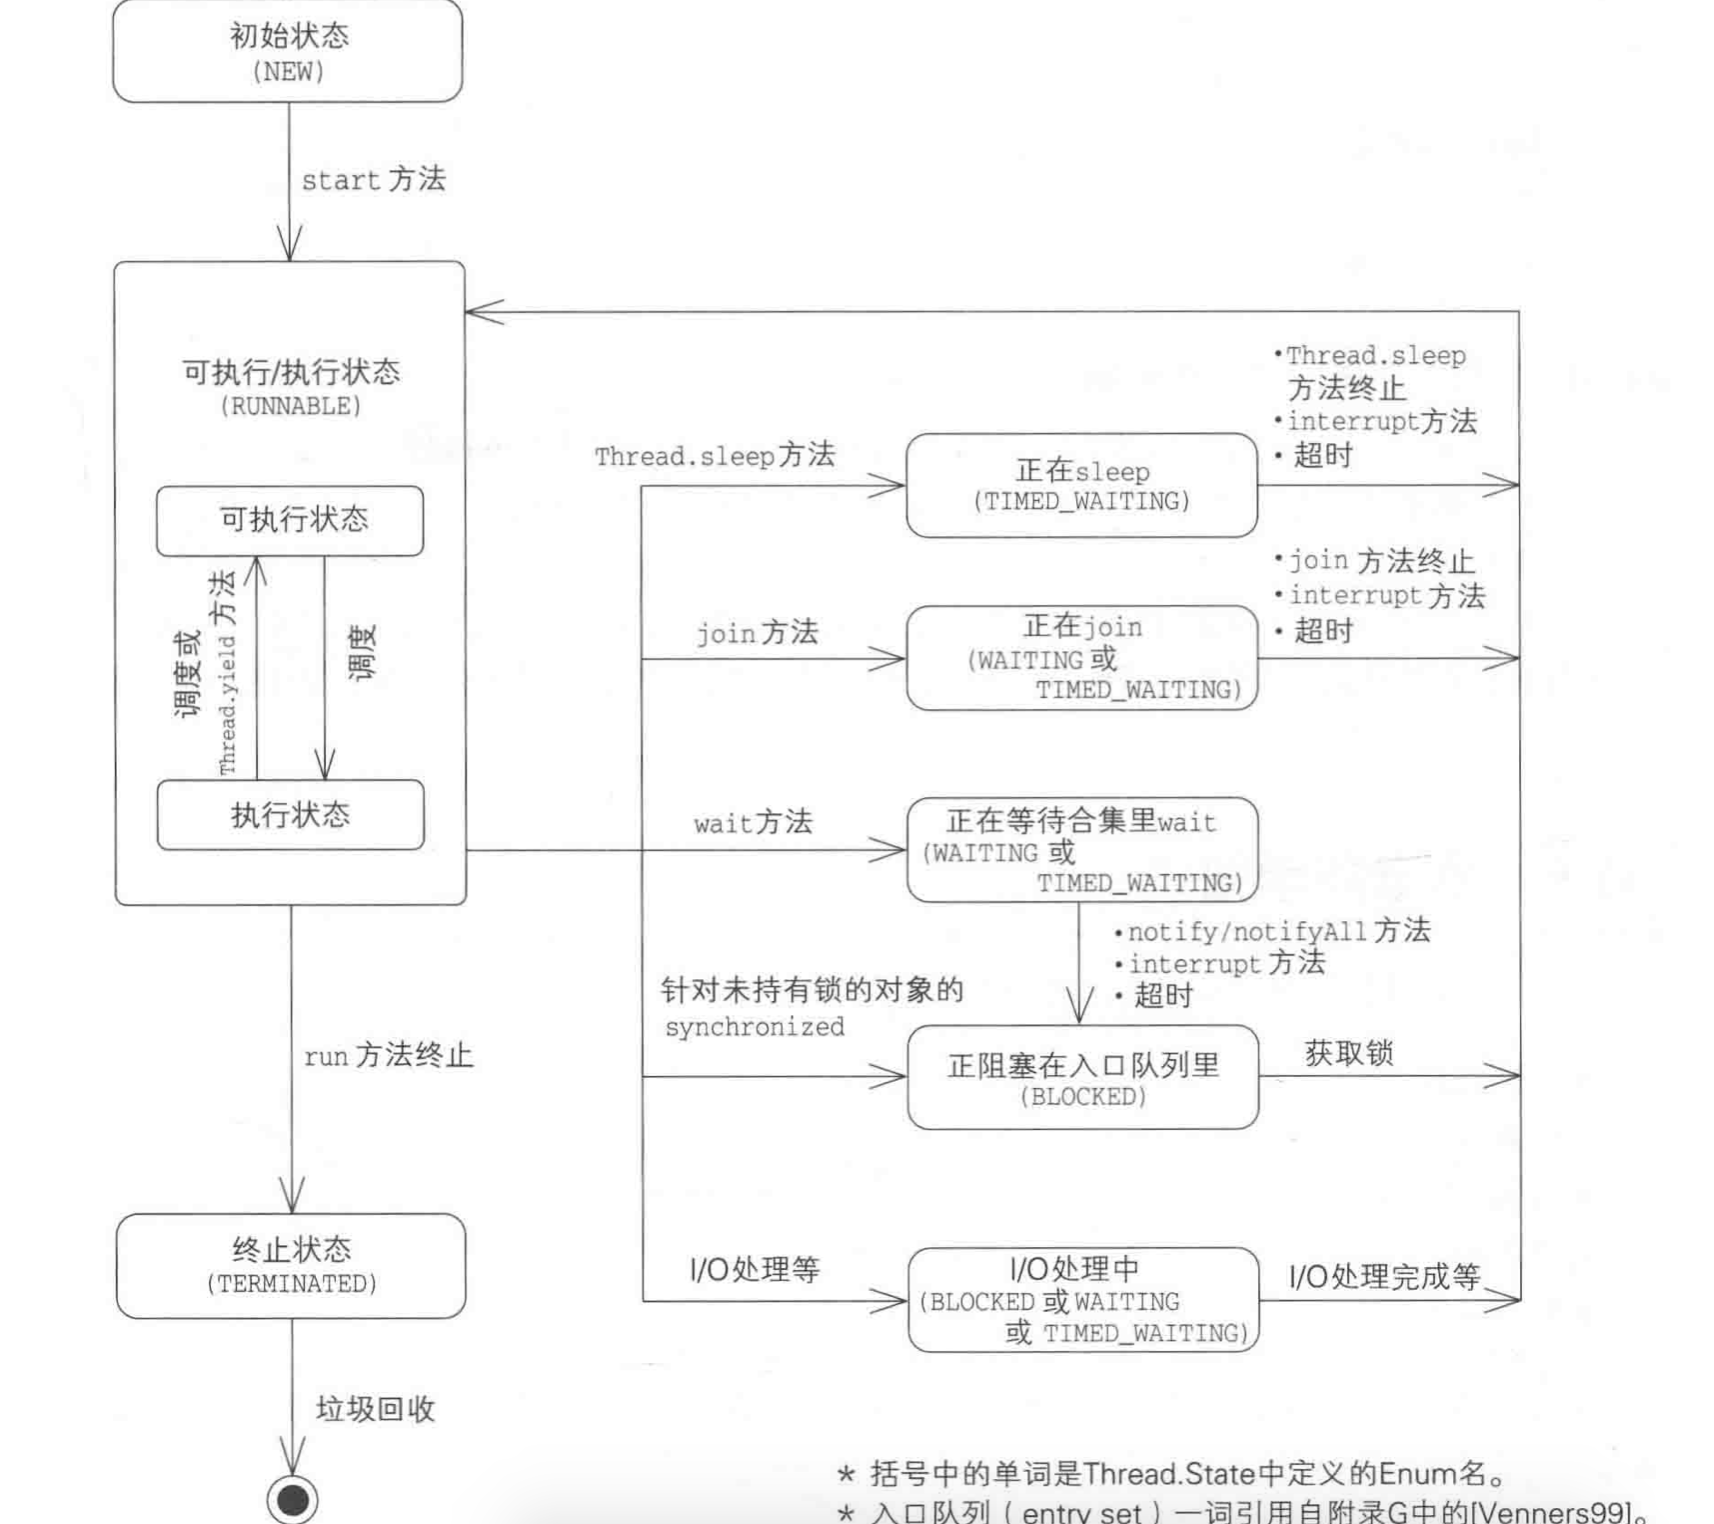
\includegraphics[width=1\textwidth]{thread/thread_states.png}
    \caption{线程状态迁移图(摘自《图解Java多线程设计模式》)}
\end{figure}

\subsubsection{NEW}

当线程被创建时,它只会短暂地处于这种状态。此时它已经分配了必须的系统资源,并执行了初始化。


\subsubsection{RUNNABLE}

只要调度器把时间片分配给线程,线程就可以运行。



下面为State枚举


\begin{lstlisting}[language=java]

public enum State {
        /**
         * 尚未启动的线程的线程状态
         */
        NEW,

        /**
         * 可运行线程的线程状态。 处于可运行状态的线程正在Java虚拟机中执行,
         * 但是它可能正在等待来自操作系统(例如处理器)的其他资源。
         */
        RUNNABLE,

        /**
         * 线程的阻塞状态,等待监视器锁定。
         * 处于阻塞状态的线程正在等待一个监视器锁进入一个同步块/方法,
         * 或者在调用Object.wait()后重新进入一个同步块/方法。
         */
        BLOCKED,

        /**
         * 等待线程状态
         * 一个线程由于调用下列方法之一而处于等待状态:
         * 
         *   Object.wait() 未超时
         *   Thread.join() 未超时
         *   LockSupport.park()
         * 
         * 处于等待状态的线程正在等待另一个线程执行特定的操作。
         * 例如: 一个线程在一个对象上已经调用了 Object.wait() ,并正在等待在另一个线程在另一对象上调用
         * Object.notify() or Object.notifyAll()。
         * 调用 thread.join() 的线程正在等待指定的线程终止。
         */
        WAITING,

        /**
         * 具有指定等待时间的等待线程的线程状态。
         * 线程处于定时等待状态,因为调用以下方法之一与指定的正等待时间:
         * 
         *   Thread.sleep()
         *   Object.wait(long)带超时参数
         *   Thread.join(long)带超时参数
         *   LockSupport.parkNanos
         *   LockSupport.parkUntil
         * 
         */
        TIMED_WAITING,

        /**
         * 终止状态。线程已经完成执行。
         */
        TERMINATED;
    }

\end{lstlisting}


\subsection{创建线程的方式}

创建线程的根本方法就是通过构造Thread类并且重写run()方法,然后调用start方法运行。

\begin{lstlisting}[language=java]

    public Thread();
    public Thread(String name);
    public Thread(ThreadGroup group, String name);

    public Thread(Runnable target);
    public Thread(Runnable target, String name);
    public Thread(ThreadGroup group, Runnable target, String name);
    public Thread(ThreadGroup group, Runnable target, String name, long stackSize);

\end{lstlisting}


创建线程有四种方式

\begin{itemize}
    \item  继承Thread类 
    \item  实现Runnable接口
    \item  实现Callable和Future接口
    \item  使用线程池方式
\end{itemize}


\subsubsection{实现Runnable接口}

Runnable接口

\begin{lstlisting}[language=java]

    @FunctionalInterface
    public interface Runnable {
        public abstract void run();
    }

\end{lstlisting}

\begin{lstlisting}[language=java]

public class HelloRunnable implements Runnable {

    public void run() {
        System.out.println("Hello from a thread!");
    }

    public static void main(String args[]) {
        (new Thread(new HelloRunnable())).start();
    }
}

\end{lstlisting}

\subsubsection{继承Thread类}

Thread类也继承了Runnable接口

\begin{lstlisting}[language=java]

    public class MyThread extends Thread {
        public void run() {
            System.out.println(Thread.currentThread().getName() + ": Run!!!");
        }
    
        public static void main(String[] args) {
            MyThread thread = new MyThread();
            thread.start();
        }
    }

\end{lstlisting}

\subsubsection{实现Callable和Future接口}

\begin{figure}[H]
    \centering
    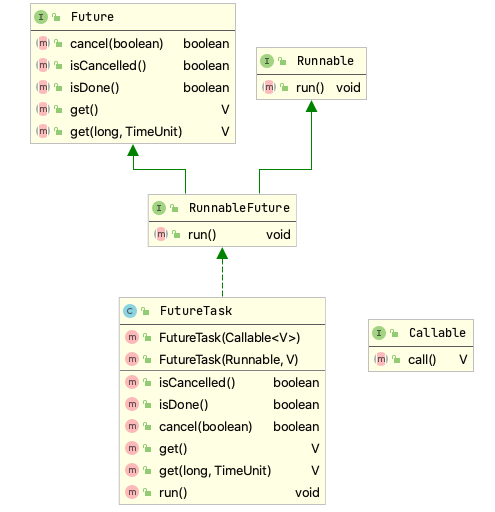
\includegraphics[width=0.8\textwidth]{thread/futuretask_diagram.png}
\end{figure}


\begin{lstlisting}[language=java]
    public class TaskWithResult implements Callable {

        private int id;
        public TaskWithResult(int id) {
            this.id = id;
        }

        @Override
        public Object call() throws Exception {
            return "Result of TaskWithResult is: " + id;
        }
    }

    public class FutureAndCallable {
    public static void main(String[] args) throws ExecutionException, InterruptedException {
        //不推荐使用Executors
        ExecutorService executorService = Executors.newCachedThreadPool();
        List<Future<String>> result = new ArrayList<>();
        for (int i = 0; i < 10; i++) {
            result.add(executorService.submit(new TaskWithResult(i)));
        }

        for (Future<String> future : result) {
            System.out.println(future.get());
        }

        executorService.shutdown();
    }
}



\end{lstlisting}


\subsubsection{使用线程池方式}

\begin{figure}[H]
    \centering
    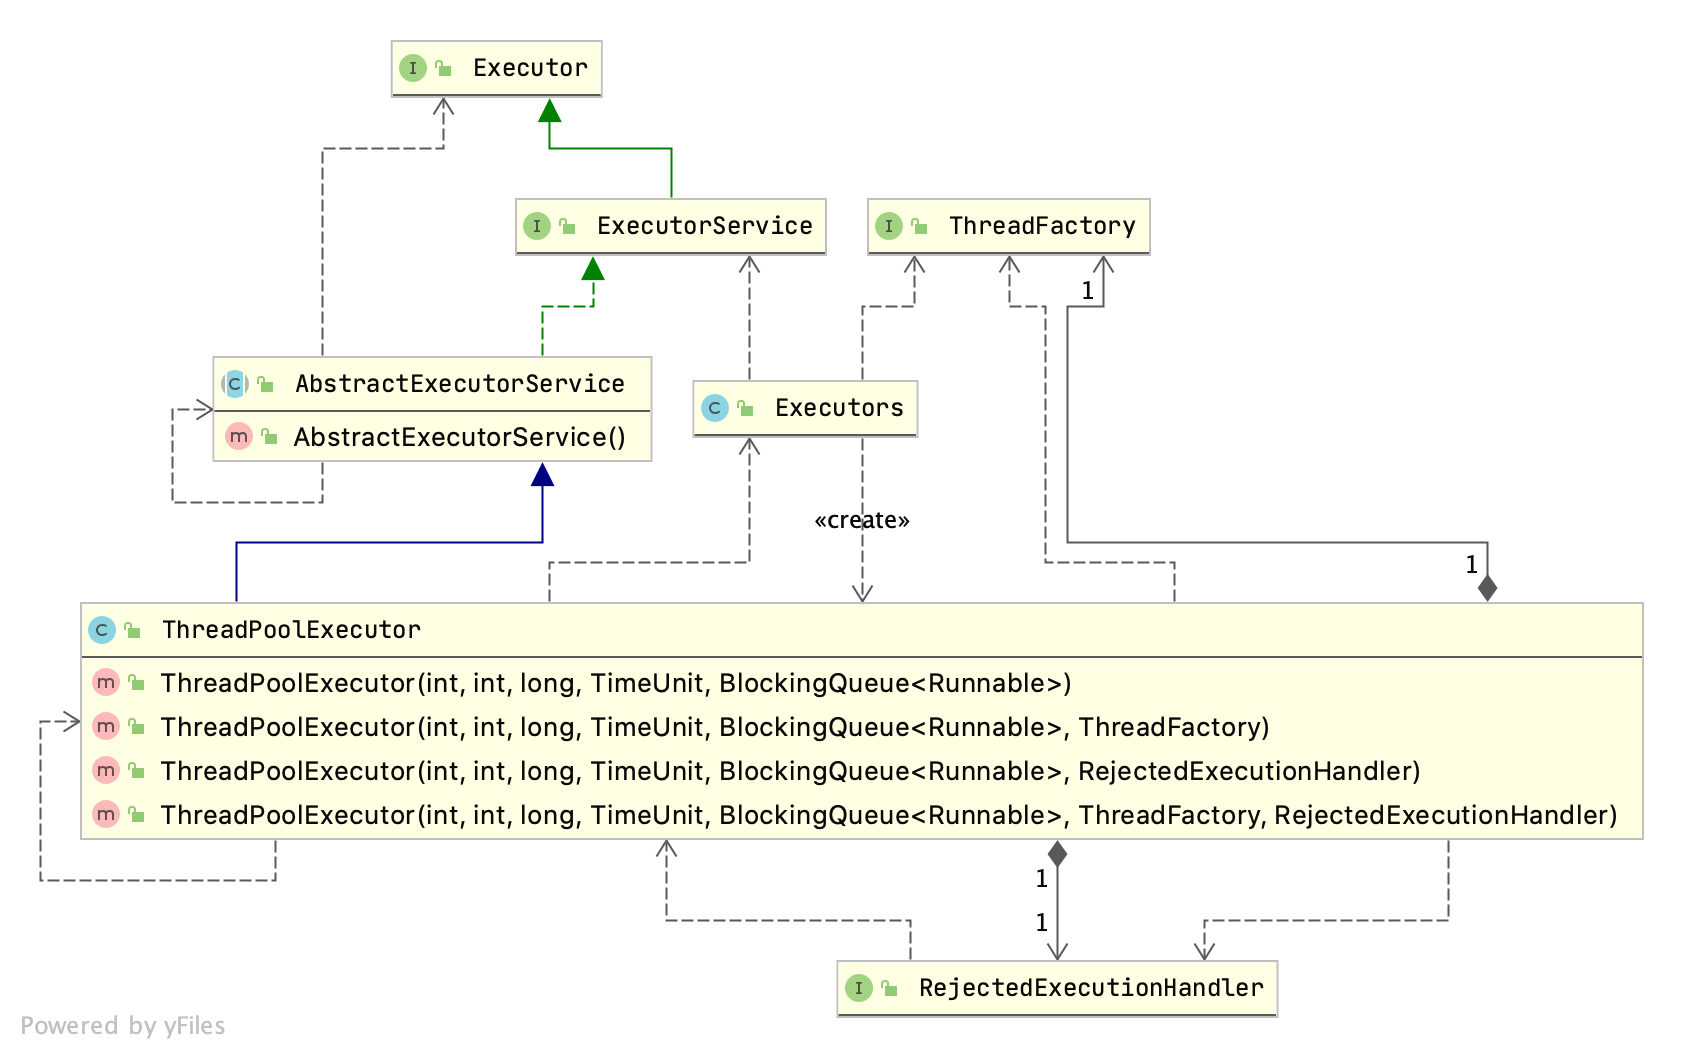
\includegraphics[width=1\textwidth]{thread/executor_diagram.png}
\end{figure}

线程池不允许使用 Executors 去创建,而是通过 ThreadPoolExecutor 的方式,这样的处理方式让写的同学更加明确线程池的运行规则,规避资源耗尽的风险。

Executors提供了如下线程池

\begin{itemize}
    \item newSingleThreadExecutor
    \item newFixedThreadPool
    \item newCachedThreadPool
    \item newScheduledThreadPool
    \item newSingleThreadScheduledExecutor
    \item newWorkStealingPool
\end{itemize}

\notebox{
    FixedThreadPool和SingleThreadExecutor:\newline
    运行的请求队列长度为Integer.MAX\_VALUE,可能会堆积大量的请求,从而导致OOM。

    CachedThreadPool:\newline
    允许的创建线程数为Integer.MAX\_VALUE,可能会创建大量的线程,从而导致OOM。
}

\begin{lstlisting}[language=java]
// 不推荐
ExecutorService executorService = Executors.newCachedThreadPool();

for (int i = 0; i < 5; i++) {
    executorService.execute(()->{
        System.out.println("Hello from a thread!");
    });
}

executorService.shutdown();

//推荐;指定最大线程数以及列队数
ExecutorService executor = new ThreadPoolExecutor(5, 5, 10L, TimeUnit.MILLISECONDS, new LinkedBlockingQueue<>(10));
for (int i = 0; i < 10; i++) {
    executor.execute(() -> System.out.println(Thread.currentThread().getName() + ":ThreadPoolExecutor"));
}

executor.shutdown();

\end{lstlisting}


\subsection{捕获异常}

不能捕获从线程中逃逸的异常。一旦异常跳出任务的run()方法,它就会向外传播到控制台。

可通过重写UncaughtExceptionHandler实现。使用setUncaughtExceptionHandler或者setDefaultUncaughtExceptionHandler方法。



\subsection{常用函数}

\begin{itemize}
    \item wait
    \item sleep
    \item join
    \item yield
    \item notify
    \item notifyAll
    \item interrupt
\end{itemize}


\subsubsection{wait}
调用wait()会释放对象上的锁。 

wait() 有两种形式。

第一种接受毫秒数做为参数,指“在此期间暂停”

在wait()期间对象锁是释放的
可以通过notify(),notifyAll()或者令时间到期,从wait()中恢复执行。

第二种不接受任何参数

wait()无限等待下去,直到线程接收到notify()或者notifyAll()的消息。

\subsubsection{sleep}
 调用sleep()的时候锁并不会被释放。

 \subsubsection{yield}
 yield()的时候锁并不会被释放。

\subsubsection{join}


wait(),notify(),notifyAll()是基类Object的一部分,而不是属于Thread的一部分。
只能在同步控制方法或者同步控制块里调用这三个方法,调用他们必须获取对象的锁。

为防止错失信号

\begin{lstlisting}[language=java]

    synchronized(sharedMonitor){
        while(someCondition){
            shareMonitor.wait();
        }
    }

\end{lstlisting}



\subsection{终止}

I/O和在synchronized块上的等待是不可中断的。















Hibernate

mybatis


\chapter{JVM}
\label{chap:jvm}




\section{javap命令}
\label{chap:javac}

Reads Java class and interface definitions and compiles them into bytecode and class files.

\begin{lstlisting}[language=cshell]
    
\end{lstlisting}
\section{javap命令}
\label{chap:tools_javap}

use the javap command to disassemble one or more class files.

\begin{lstlisting}[language=cshell]

用法: javap <options> <classes>

  -version                 版本信息
  -v  -verbose             输出附加信息
  -l                       输出行号和本地变量表
  -public                  仅显示公共类和成员
  -protected               显示受保护的/公共类和成员
  -package                 显示程序包/受保护的/公共类和成员 (默认)
  -p  -private             显示所有类和成员
  -c                       对代码进行反汇编
  -s                       输出内部类型签名
  -sysinfo                 显示正在处理的类的系统信息 (路径, 大小, 日期, MD5 散列)
  -constants               显示最终常量
  -classpath <path>        指定查找用户类文件的位置
  -cp <path>               指定查找用户类文件的位置
  -bootclasspath <path>    覆盖引导类文件的位置

\end{lstlisting}

示例:

\begin{lstlisting}[language=java]

javap -c Main.class

\end{lstlisting}

\subsection{Java字节码} 

Instruction set 


instructions fall into a number of broad groups:

\begin{itemize}
    \item 加载和存储指令(Load and store)(e.g. aload\_0, istore)
    \item 算术与逻辑指令(Arithmetic and logic) (e.g. ladd, fcmpl)
    \item 类型转换指令(Type conversion) (e.g. i2b, d2i)
    \item 对象创建与操作指令(Object creation and manipulation) (new, putfield)
    \item 堆栈操作指令(Operand stack management) (e.g. swap, dup2)
    \item 控制转移指令(Control transfer) (e.g. ifeq, goto)
    \item 方法调用与返回指令(Method invocation and return) (e.g. invokespecial, areturn)
\end{itemize}

大多数的指令有前缀和(或)后缀来表明其操作数的类型。如下表:

Many instructions have prefixes and/or suffixes referring to the types of operands they operate on.

\begin{table}[H]
    \centering
    \caption{前缀/后缀类型对照表}
    \begin{tabular}{|l|l|}
    \hline
    Prefix/suffix & Operand type    \\ \hline
    i           & integer           \\ \hline
    l           & long             \\ \hline
    s           & short             \\ \hline
    b           & byte              \\ \hline
    c           & character         \\ \hline
    f           & float             \\ \hline
    d           & double            \\ \hline
    a           & reference         \\ \hline
    \end{tabular}
    \end{table}


Java bytecode

\begin{table}[H]
    \centering
    \caption{Java字节码}
    \begin{tabular}{|l|l|l|}
    \hline
    mnemonic    & stack [before]->[after]   & description                                           \\ \hline
    aload\_0    & → objectref               & load a reference onto the stack from local variable 0  \\ \hline
    \end{tabular}
    \end{table}


        
\href{https://en.wikipedia.org/wiki/Java_bytecode_instruction_listings}{bytecode}

\href{http://blog.jamesdbloom.com/JavaCodeToByteCode_PartOne.html}{code}

\href{https://docs.oracle.com/javase/specs/jvms/se8/html/jvms-4.html#jvms-4.10.1.9}{jvms}
  
\section{java命令}
\label{chap:tools_java}

Launches a Java application.

\begin{lstlisting}[language=cshell]

    java [options] classname [args]

    java [options] -jar filename [args]

\end{lstlisting}

通过启动JRE来调用指定的类,调用此类的main()方法。
\begin{lstlisting}[language=Java]
    public static void main(String[] args)
\end{lstlisting}

\subsection{选项} 


\begin{itemize}
    \item   标准选项
    \item   非标准选项 
    \item   高级运行时选项      (Advanced Runtime Options)
    \item   高级JIT编译器选项   (Advanced JIT Compiler Options)
    \item   高级可维护性选项    (Advanced Serviceability Options)
    \item   高级垃圾收集选项    (Advanced Garbage Collection Options)
\end{itemize}



\subsubsection{标准选项} 

Java虚拟机(JVM)的所有实现都保证支持的标准选项。


* -agentlib:libname[=options]

加载指定的本机代理库。在库名之后,可以使用特定于库的以逗号分隔的选项列表。

如果指定 -agentlib:foo 选项,则JVM尝试加载位于由系统环境变量名为LD\_LIBRARY\_PATH(在OS X系统下变量名为 DYLD\_LIBRARY\_PATH)指定位置下的libfoo.so的库。

下面的示例将展示如何加载堆分析工具(HPROF)库,并且获取堆栈深度为3,每20msCPU的简单采样信息:

\begin{lstlisting}[language=cshell]

    -agentlib:hprof=cpu=samples,interval=20,depth=3

\end{lstlisting}  

下面这个示例将展示如何加载Java调试线协议库并且监听8000端口的套接字连接,在主类加载之前挂起JVM:


\begin{lstlisting}[language=cshell]

    -agentlib:jdwp=transport=dt_socket,server=y,address=8000

\end{lstlisting} 





\-XX:+PrintStringTableStatistics



\section{jps命令}
\label{chap:tools_jps}

Lists the instrumented Java Virtual Machines (JVMs) on the target system. 

只适用于HotSpot虚拟机。

\begin{lstlisting}[language=cshell]

jps [ options ] [ hostid ]

\end{lstlisting}

hostid可以是进程的标识符或者类似于URL的 [protocol:][[//]hostname][:port][/servername] 地址

如果jps命令没有指定hostid参数,那么工具只搜索本机运行的JVM。如果指定了hostid,那么他将通过指定的地址来搜索JVM。
使用指定hostid的主机必须运行着jstatd进程。

\subsection{选项} 

\menlo{-q}

只输出JVM标识符的列表,不输出类名、JAR文件名以及传递给main方法的参数。


\menlo{-m}

输出传递给mian方法的参数。嵌入式JVMS可能输出为空。


\menlo{-l}

输出应用程序主类的完整包名或应用程序JAR文件的完整路径名。

\menlo{-v}

输出传递给JVM的参数。

\menlo{-V}

只输出本地JVM标识符,不输出类名、JAR文件以及传递给main方法的参数。


\menlo{-Joption}

将选项传递给JVM,其中的选项是Java应用程序启动程序参考页面中描述的选项之一。例如,-J-Xms48m将启动内存设置为48 MB。



输出格式:

\begin{lstlisting}[language=cshell]

lvmid [ [ classname | JARfilename | "Unknown"] [ arg* ] [ jvmarg* ] ]

\end{lstlisting}



示例:

\begin{lstlisting}[language=cshell]
jps

    18027 Java2Demo.JAR
    18032 jps
    18005 jstat

\end{lstlisting}


\begin{lstlisting}[language=cshell]

jps -m remote.domain:2002

       3002 /opt/jdk1.7.0/demo/jfc/Java2D/Java2Demo.JAR
       3102 sun.tools.jstatd.jstatd -p 2002

    \end{lstlisting}
\section{jcmd命令}
\label{chap:tools_jcmd}

Sends diagnostic command requests to a running Java Virtual Machine (JVM).

\begin{lstlisting}[language=cshell]

    jcmd [-l|-h|-help]

    jcmd pid|main-class PerfCounter.print

    jcmd pid|main-class -f filename

    jcmd pid|main-class command[ arguments]

\end{lstlisting}


jcmd工具向JVM发送诊断命令请求。必须在当前运行着JVM机器上执行,并且具有与JVM具有相同的user和group标识。

运行jcmd不带参数或者使用 \-l 选项时,相当于jps (\textcolor[rgb]{0,0,1}{\ref{chap:tools_jps}}),会输出java进程标识符。

如果将进程标识符(pid)或主类(main-class)作为第一个参数,则jcmd将诊断命令请求发送给具有指定标识符或发具有指定main-class名称的Java进程。

如果使用0作为进程标识符,则会将诊断命令请求发送给所有可用的Java进程。


* Perfcounter.print

打印指定Java进程可用的性能计数器。性能计数器的列表可能因Java进程而异。


* -f filename

从文件中读取诊断命令。文件中每个命令必须单独一行。以\# 开头的命令会被忽略。如果命令行中包含\textcolor{codepurple}{stop}关键字则结束命令行读取。

* command [arguments]

要发送到指定Java进程的命令。可以通过向该进程发送\textcolor{codepurple}{help}命令来获得给定进程的可用诊断命令列表。

如果参数中包含空格,则必须使用单引号或者双引号扩起来。注意使用转义字符($\backslash$)转义单/双引号。


\begin{lstlisting}[language=cshell]

   jcmd 15 help     # 15为java进程id

    #### output ####

    15:
    The following commands are available:
    JFR.stop
    JFR.start
    JFR.dump
    JFR.check
    VM.native_memory
    VM.check_commercial_features
    VM.unlock_commercial_features
    ManagementAgent.stop
    ManagementAgent.start_local
    ManagementAgent.start
    VM.classloader_stats
    GC.rotate_log
    Thread.print
    GC.class_stats
    GC.class_histogram
    GC.heap_dump
    GC.finalizer_info
    GC.heap_info
    GC.run_finalization
    GC.run
    VM.uptime
    VM.dynlibs
    VM.flags
    VM.system_properties
    VM.command_line
    VM.version
    help

\end{lstlisting}

\begin{lstlisting}[language=cshell]
    jcmd 15 help GC.heap_info
\end{lstlisting}








\chapter{内存模型}
\label{chap:memory}

\section{Java内存模型与线程}
 
\begin{figure}[H]
    \centering
    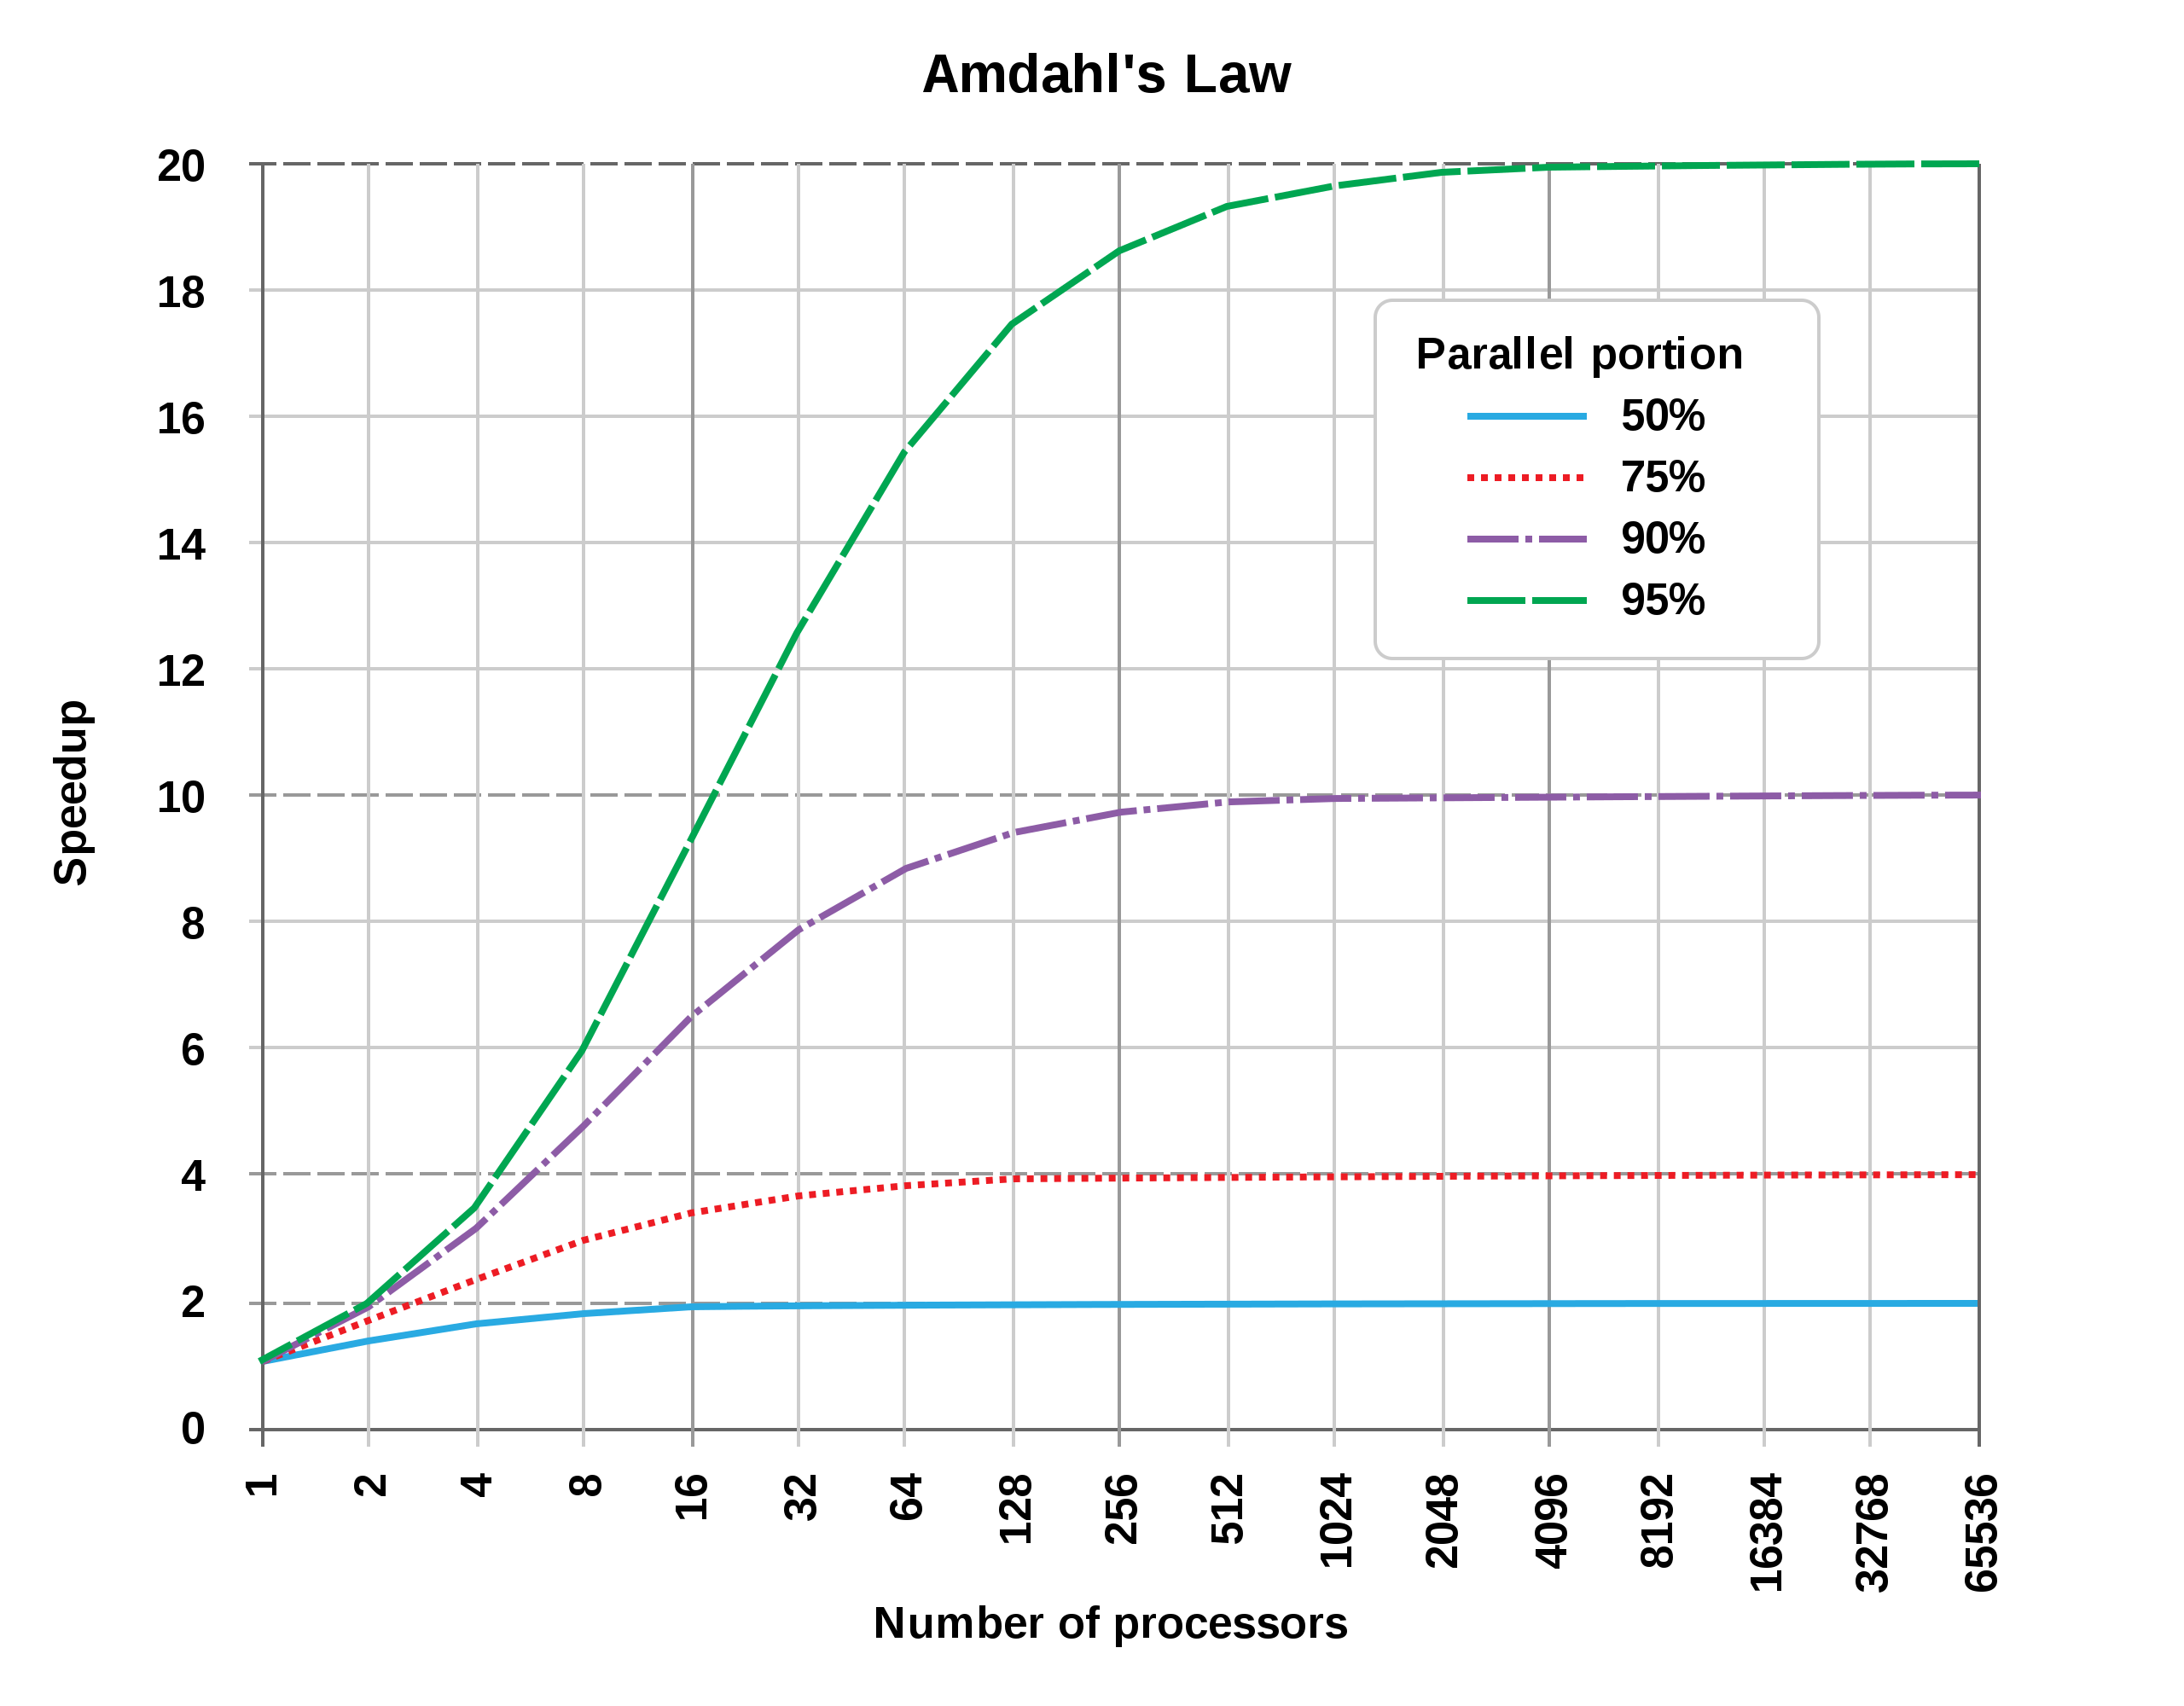
\includegraphics[width=0.8\textwidth]{parallel/amdahls-law-0.png}
    \caption{Amdahl's Law 阿姆达尔定律}
\end{figure}

并发不得不知的阿姆达定律。

一个程序(或者一个算法)可以按照是否可以被并行化分为下面两个部分:

\begin{itemize}
    \item 可以被并行化的部分
    \item 不可以被并行化的部分 
\end{itemize}


程序串行执行的总时间我们记为\textbf{T}。

时间\textbf{T}包括:不可以被并行和可以被并行部分的时间。不可以并行的部分记为\textbf{B}, 可以被并行的部分就是\textbf{T} - \textbf{B}。即 \textbf{T} = \textbf{B} + (\textbf{T} – \textbf{B}) 

定义如下:

\begin{lstlisting}

 T = 串行执行的总时间

 B = 不可以并行的总时间

 T - B = 并行部分的总时间

\end{lstlisting}


\textbf{T} - \textbf{B} 是可并行化的部分,以并行的方式执行可以提高程序的执行速度。可以提速多少取决于有多少线程或者多少个CPU来执行。线程或者CPU的个数我们记为\textbf{N}。可并行化部分被执行的最快时间可以通过下面的公式计算出来:

(\textbf{T} – \textbf{B} ) / \textbf{N} 或 (1/\textbf{N}) * (\textbf{T} - \textbf{B})

根据阿姆达定律,当可并行部分使用`N`个线程或CPU执行时,程序的总执行时间为:

\textbf{T}(\textbf{N}) = \textbf{B} + (\textbf{T} - \textbf{B}) / \textbf{N}

\notebox{T(N)表示并行因子为N的总执行时间。T(1)就是并行因子为1时的总执行时间。 T(N) = B + (T(1) – B) / N }


示例

\begin{lstlisting}
/*
 * 总时间为1。串行时间为0.4,那么并行时间为0.6。
 */

// 并行因子为2时
T(2) = 0.4 + ( 1 - 0.4 ) / 2
 = 0.4 + 0.6 / 2
 = 0.4 + 0.3
 = 0.7

// 并行因子为5时
 T(5) = 0.4 + ( 1 - 0.4 ) / 5
 = 0.4 + 0.6 / 6
 = 0.4 + 0.12
 = 0.52
\end{lstlisting}

图示

并行因子分别为1,2,3时。

\begin{figure}[H]
    \centering
    \subfigure[并行因子=1]{
        \label{P1}
        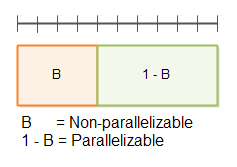
\includegraphics[width=0.45\textwidth]{parallel/amdahls-law-1.png}}
    \subfigure[并行因子=2]{
        \label{P2}
        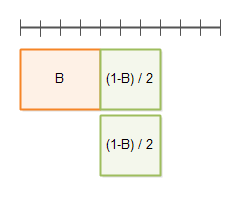
\includegraphics[width=0.45\textwidth]{parallel/amdahls-law-2.png}}
        \caption{并行因子分别为1,2时}
\end{figure}

\begin{figure}[H]
    \centering
    \label{P3}
    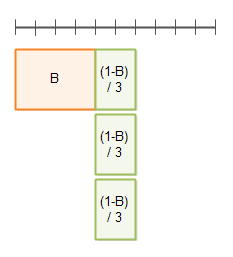
\includegraphics[width=0.8\textwidth]{parallel/amdahls-law-3.png}
    \caption{并行因子=3}
\end{figure}


\subsubsection{定义} 

并行计算中的\textbf{加速比}是用并行前的执行速度和并行后的执行速度之比来表示的,它表示了在并行化之后的效率提升情况。


 \begin{figure}[H]
    \centering
    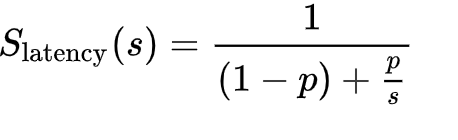
\includegraphics[width=1\textwidth]{parallel/amdahls-definition.png}
    \caption{阿姆达尔定律}
\end{figure}

S(latency)代表理论上的加速比

s 为并行处理结点个数

p 为并行计算部分所占比例

1-p为串行计算部分所占比例

这样:

当p = 1时,最大加速比p = s,

当p = 0时,最小加速比S = 1,

当 s→∞ 时,极限加速比S→ 1/(1-p),这也就是加速比的上限。

例如,若加速前并行代码执行时间占整个代码的执行时间的75%(p=0.75),则加速后并行处理的总体性能的提升不可能超过原先的4倍。

因此可以推断出:

 \begin{figure}[H]
    \centering
    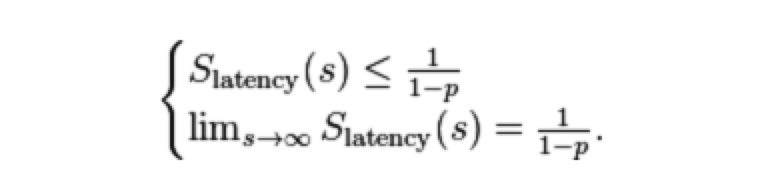
\includegraphics[width=1\textwidth]{parallel/amdahls-definition-1.png}
    \caption{阿姆达尔定律}
\end{figure}

阿姆达尔定律强调:当串行换比例一定时,加速比是有上限的,不管你堆叠多少个CPU参与计算,都不能突破这个上限。


\subsection{Gustafson's law 古斯塔夫森定律}


 \begin{figure}[H]
    \centering
    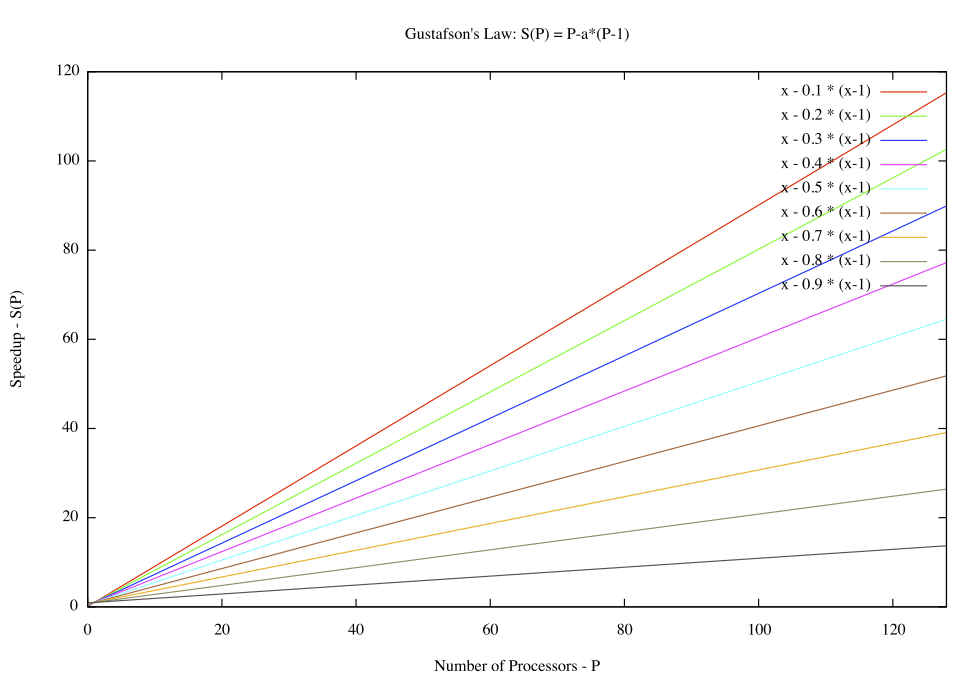
\includegraphics[width=1\textwidth]{parallel/gustafson.png}
    \caption{古斯塔夫森定律}
\end{figure}

 \begin{figure}[H]
    \centering
    
\includegraphics[width=1\textwidth]{parallel/gustafson-definition.png}
    \caption{古斯塔夫森定律定义}
\end{figure}

古斯塔夫森定律强调的是:如果可被并行化的代码所占比例足够大,那么加速比就能随着CPU的数量线性增长。



\subsection{JAVA内存模型 JMM}

JAVA内存模型 Java Memory Model JMM














% linux
\chapter{JVM}
\label{chap:jvm}




\section{uptime}
\label{chap:linux_uptime}

uptime

当前时间系统运行了多长时间、多少用户登陆;以及过去1分钟、5分钟、15分钟的系统平均负载。

\begin{lstlisting}[language=cshell]
    $ uptime

    # 20:08:43 up 11 days,  6:06,  0 users,  load average: 21.76, 21.24, 19.93

    # 20:08:43      系统当前时间
    # up 11 days,  6:06     系统运行时间
    # 0 users       当前登陆用户数
    # load average: 21.76, 21.24, 19.93     过去1分钟、5分钟、15分钟的系统平均负载
\end{lstlisting}


系统负载

系统负载是处于可运行(runnable)或不可中断(uninterruptable)状态的进程的平均数。\par
可运行(runnable)状态的进程要么正在使用CPU,要么在等待使用CPU。不可中断状态的进程则正在等待某些I/O访问,例如等待磁盘IO。 \par
负载均值的意义根据系统中 CPU 的数量不同而不同,负载为 1 对于一个只有单 CPU 的系统来说意味着负载满了,而对于一个拥有 4 CPU 的系统来说则意味着 75\% 的时间里都是空闲的。


\par
OPTIONS

-p, --pretty \par
\qquad 以漂亮的格式显示正常运行时间

\begin{lstlisting}[language=cshell]
    uptime -p

    # up 17 weeks, 1 day, 11 hours, 37 minutes
\end{lstlisting}


-s, --since \par
\qquad 以yyyy-mm-dd HH:MM:SS格式显示系统启动时间

\begin{lstlisting}[language=cshell]
    uptime -s

    # 2019-11-18 23:30:43
\end{lstlisting}













\section{top}
\label{chap:linux_top}

显示Linux进程信息

top提供了运行系统的动态实时视图。它可以显示系统摘要信息以及当前由Linux内核管理的进程或线程的列表。所显示的系统摘要信息的类型以及为流程显示的信息的类型、顺序和大小都是用户可配置的
该配置可以在重启时保持不变。


下文以3.3.10版本为例。

\subsection{交互式命令}

进入top命令页面后输入的命令

\menlo{l}     切换是否显示系统平均负载

\menlo{c}     切换程序名或命令行的显示

\menlo{d}     修改屏幕刷新时间

\menlo{i}     切换显示所以线程或任务

\menlo{H}     切换为线程模式

\menlo{t}     切换Task/Cpu显示状态

\menlo{m}     切换内存模式显示状态

\menlo{f}     增加/删除/排序字段

\menlo{1/2/3}   切换展示所有CPU/numa/node使用情况

\menlo{L}    查找

\menlo{E/e}  概括/线程内存预览

\menlo{S}    切换累积模式


\subsection{OPTIONS}

-b  \par
\qquad 批处理模式操作,可用于将top输出内容发送到其他程序或者文件中

-c \par 
\qquad 显示完整命令行或者程序名

-d :Delay-time interval as:  -d ss.t (secs.tenths)  \par 
\qquad  指定屏幕更新时间间隔;也可以使用交互命令d或者s。可以填写分数秒。

-H  :Threads-mode operation \par
\qquad  指定显示各个线程,如果没有此选项,则显示每个进程中所有线程的总和。也可以使用交互命令H。

-i  :Idle-process toggle    \par 
\qquad 使top不显示任何闲置或者僵死进程。

-n  :Number-of-iterations limit as:  -n number  \par 
\qquad  循环显示的次数

-o  :Override-sort-field as:  -o fieldname  \par
\qquad 指定将对那些任务字段进行排序。可以在字段名前加上+或者-用来覆盖排序方向。前置+将强制从高到低排序,而-是从低到高排序。可用字段名可以参选下面的-O选项。

-O  :Output-field-names \par
\qquad 打印可用的字段名

-p  :Monitor-PIDs mode as:  -pN1 -pN2 ...  or  -pN1,N2,N3 ...\par
\qquad 仅监视具有指定进程id的进程。此选项最多可以使用20次,或者您可以提供最多20个pid的逗号分隔列表。如果需要恢复,可以使用=,u或U。

-S  :Cumulative-time toggle \par
\qquad 当启用累积时间模式时,每个进程都会列出它和它死去的子进程所使用的cpu时间。

-u | -U  :User-filter-mode as:  -u | -U number or name\par 
\qquad 只显示与给定的用户id或用户名匹配的进程。-u选项匹配有效用户,而-U选项匹配任何用户(实际的、有效的、已保存的或文件系统)。在用户id或名称前面加上感叹号('!'),指示top只显示与提供的用户不匹配的进程。


输出内容解释

\begin{figure}[H]
    \centering
    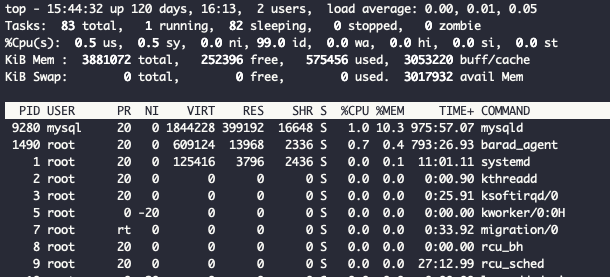
\includegraphics[width=1\textwidth]{linux/top-1.png}
    \caption{top}
\end{figure}


第一行输出任务为UPTIME and LOAD Averages

\begin{lstlisting}[language=cshell]

#   top - 15:52:24 up 120 days, 16:21,  2 users,  load average: 0.14, 0.10, 0.07

\end{lstlisting}

第二行为任务(进程)或者线程信息;进程或者线程的切换可以通过交互命令H。 分为:运行;休眠;停止;僵尸

\begin{lstlisting}[language=cshell]

#   Tasks:  86 total,   1 running,  85 sleeping,   0 stopped,   0 zombie

#   Threads: 149 total,   1 running, 148 sleeping,   0 stopped,   0 zombie

\end{lstlisting}


第三行为CPU状态信息


\begin{lstlisting}[language=cshell]

#   %Cpu(s):  0.7 us,  0.7 sy,  0.0 ni, 98.7 id,  0.0 wa,  0.0 hi,  0.0 si,  0.0 st
#              a   b      c  d 
#   %Cpu(s):  0.3/0.5     1[|

\end{lstlisting}

us, user    : 用户空间占用CPU百分比(time running un-niced user processes)    \par
sy, system  : 内核空间占用CPU百分比(time running kernel processes)  \par
ni, nice    : 用户进程空间内改变过优先级的进程占用CPU百分比(time running niced user processes)   \par
id, idle    : 空闲CPU百分比(time spent in the kernel idle handler)  \par
wa, IO-wait : 等待输入输出的CPU时间百分比(time waiting for I/O completion)       \par
hi : 硬中断(Hardware IRQ)占用CPU的百分比(time spent servicing hardware interrupts)      \par
si : 软中断(Software Interrupts)占用CPU的百分比(time spent servicing software interrupts)      \par
st : hypervisor vm占用的CPU时间的百分比(time stolen from this vm by the hypervisor) \par

在使用交互命令t切换到cpu状态模式时,还会额外显示一行CPU摘要信息,如上面展示第二行

a) 是 us 和 ni 之和 \par
b) 是 sy 百分比 \par
c) 是总和   \par
d) 是可视化图像 \par


内存使用情况

默认情况下,第1行反映物理内存,分类为:\par
total(物理内存总量), free(空闲内存总量), used(使用的物理内存总量) and buff/cache(用作内核缓存的内存量)

第2行反映的主要是虚拟内存,分为以下几类:\par
total(交换区总量), free(闲交换区总量), used(使用的交换区总量) and avail(可用物理内存)

此行的avail 指启动新应用程序时可用的物理内存的估计值不包含swapping。与free命令不同的是,free试图分析易于回收的页面缓存和内存片。

可以通过交互命令E切换单位

\begin{lstlisting}[language=cshell]

# MiB Mem :   3790.1 total,    228.7 free,    568.1 used,   2993.2 buff/cache
# MiB Swap:      0.0 total,      0.0 free,      0.0 used.   2941.0 avail Mem

\end{lstlisting}

在内存模式(使用交互命令m)下,会显示两行简短的简要:

\begin{lstlisting}[language=cshell]

            a    b          c
MiB Mem : 23.2/3790.1   [|||||                         ]
MiB Swap:  0.0/0.0      [                              ]

\end{lstlisting}

a) 使用百分比

b) 总物理内存

c) 图形化展示


\begin{lstlisting}[language=cshell]

PID USER      PR  NI    VIRT    RES    SHR S  %CPU %MEM     TIME+ COMMAND
9280 mysql     20   0 1844228 399192  16648 S   0.7 10.3 990:08.75 mysqld
1490 root      20   0  609124  13968   2336 S   0.3  0.4 803:34.96 barad_agent

\end{lstlisting}

\subsection{列字段含义}

1. \%CPU  -- CPU使用率  \par
\qquad CPU使用时间占比;

2. \%MEM  --  内存使用 (RES)   \par
\nftt{进程当前使用的可用物理内存占比}

3. CGROUPS  --  Control Groups  \par

4. CODE  --  Code Size (KiB) \par
\nftt{可执行代码占用物理内存大小,也称为文本常驻集(Text Resident Set)大小或TRS。}

5. COMMAND  --  命令名/命令行   \par

6. DATA  --  Data + Stack Size (KiB) 数据段 + 栈    \par
\nftt{可执行代码以外的物理内存的大小,也称为数据常驻集大小或DRS。}

7. ENVIRON  --  环境变量   \par

8. Flags  --  Task Flags    \par
\nftt{This column represents the task's current scheduling flags which are expressed in hexadecimal notation and with zeros suppressed.  These flags are officially documented in <linux/sched.h>.}

9. GID  --  有效组ID \par

10. GROUP  --  有效组名 \par

11. NI  --  Nice Value 进程的nice值。nice值越小优先级越高。 0表示不调整优先级。  \par

12. P  --  Last used CPU (SMP)  \par
\nftt{A number representing the last used processor.  In a true SMP environment this will likely change frequently since the kernel intentionally uses weak affinity.  Also, the very act of running top may break this weak affinity and cause  more  processes  to
change CPUs more often (because of the extra demand for cpu time).}

13. PGRP  --  进程组ID  \par

14. PID  --  进程ID \par

15. PPID  --  父进程ID \par

16. PR  --  优先级   \par

\nftt{进程调度优先级。如果在字段中看到rt,则说明该线程正在实时调度优先级下运行。}

17. RES  --  进程占用内存大小 (KiB) \par
\nftt{进程使用的未被swap物理内存大小(The non-swapped physical memory a task is using.)}

18. RUID  --  真实用户id \par

19. RUSER  --  真实用户名 \par

20. S  --  进程状态(Process Status) \par
\begin{itemize}
    \item \nftt{ D = 不可中断睡眠状态(uninterruptible sleep) }
    \item \nftt{ R = 运行状态(running)   }
    \item \nftt{ S = 睡眠状态(sleeping) }
    \item \nftt{ T = stopped by job control signal  }
    \item \nftt{ t = stopped by debugger during trace   }
    \item \nftt{ Z = 僵尸状态(zombie)   }
\end{itemize}

\nftt{D状态一般为等待IO,例如磁盘IO、网络IO等。}

21. SHR  --  共享内存大小(Shared Memory Size) (KiB)   \par
\nftt{进程可用的共享内存大小,通常不是所有的都驻留。它只能反应可能与其他进程共享的内存。}

22. SID  -- 会话ID \par

23. SUID  --  Saved User Id \par

24. SUPGIDS  --  附属组ID    \par

25. SUPGRPS  --  附属组名  \par

26. SUSER  --  Saved User Name  \par

27. SWAP  --  Swapped Size (KiB)  线程地址空间的非驻留部分  \par

28. TGID  --  线程组ID(Thread Group Id) \par
\nftt{任务所属的线程组的ID。它是线程组领导的PID。在内核术语中,它表示那些共享mm\_struct的任务。}

29. TIME  --  CPU Time  \par
\nftt{线程启动后使用的总CPU时间。当启用累积模式时,将列出每个进程以及其死去的字进程所使用的CPU时间。可以使用交互命令S来切换累积模式。}

30. TIME+  --  CPU Time, hundredths \par
\nftt{与TIME相同,但通过百分之一秒反映出更细的粒度。}

31. TPGID  --  Tty Process Group Id \par

32. TTY  --  Controlling Tty    \par

33. UID  --  用户ID;进程所有者的真实用户ID   \par

34. USED  --  Memory in Use (KiB)   \par
\nftt{此字段表示线程使用的非swapped物理内存(RES)及其地址空间的非驻留部分(SWAP)。}

35. USER  --  用户名;进程所有者的真实用户名  \par

36. VIRT  --  虚拟内存大小(Virtual Memory Size)(KiB) \par
\nftt{进程使用的虚拟内存大小。包括代码,数据以及共享库以及已换出的页和已映射但未使用的页。}

37. WCHAN  --  Sleeping in Function \par
\nftt{若该进程在睡眠,则显示睡眠中的系统函数名。}

38. nDRT  --  脏页数量(Dirty Pages Count) \par
\nftt{The number of pages that have been modified since they were last written to auxiliary storage.  Dirty pages must be written to auxiliary storage before the corresponding physical memory location can be used for some other virtual page.}

39. nMaj  --  Major Page Fault Count    \par
\nftt{The number of major page faults that have occurred for a task.  A page fault occurs when a process attempts to read from or write to a virtual page that is not currently present in its address space.  A major page fault is when auxiliary  storage  access
is involved in making that page available.}

40. nMin  --  Minor Page Fault count    \par
\nftt{The number of minor page faults that have occurred for a task.  A page fault occurs when a process attempts to read from or write to a virtual page that is not currently present in its address space.  A minor page fault does not involve auxiliary storage
access in making that page available.}

41. nTH  --  线程数量  \par

42. nsIPC  --  IPC namespace    \par
\nftt{The Inode of the namespace used to isolate interprocess communication (IPC) resources such as System V IPC objects and POSIX message queues.}

43. nsMNT  --  MNT namespace    \par
\nftt{The Inode of the namespace used to isolate filesystem mount points thus offering different views of the filesystem hierarchy.}

44. nsNET  --  NET namespace    \par
\nftt{The Inode of the namespace used to isolate resources such as network devices, IP addresses, IP routing, port numbers, etc.}

45. nsPID  --  PID namespace    \par
\nftt{The Inode of the namespace used to isolate process ID numbers meaning they need not remain unique.  Thus, each such namespace could have its own `init' (PID \#1) to manage various initialization tasks and reap orphaned child processes.}

46. nsUSER  --  USER namespace  \par
\nftt{The Inode of the namespace used to isolate the user and group ID numbers.  Thus, a process could have a normal unprivileged user ID outside a user namespace while having a user ID of 0, with full root privileges, inside that namespace.}

47. nsUTS  --  UTS namespace    \par
\nftt{The Inode of the namespace used to isolate hostname and NIS domain name.  UTS simply means "UNIX Time-sharing System".}

48. vMj  --  Major Page Fault Count Delta   \par
\nftt{The number of major page faults that have occurred since the last update (see nMaj).}

49. vMn  --  Minor Page Fault Count Delta   \par
\nftt{The number of minor page faults that have occurred since the last update (see nMin).}


\subsection{示例}

\begin{figure}[H]
    \centering
    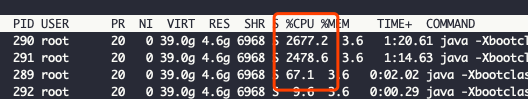
\includegraphics[width=1\textwidth]{linux/top_cpu_over_100.png}
    \caption{top cpu利用率超过100\%}
\end{figure}

\subsubsection{如上图所示:CPU使用率超过100\%}

这里CPU使用率是所有CPU的总和。即你的CPU是多核处理器。可以使用交互式命令1来查看所有CPU的使用情况。










\section{free}
\label{chap:linux_free}

显示系统中空闲和使用的物理内存以及swap内存量。还有内核使用的缓冲区和缓存。这些信息来源于/proc/meminfo。

total   \par
\nftt{总内存大小 (MemTotal and SwapTotal in /proc/meminfo)}

used    \par   
\nftt{已使用的内存大小 (calculated as total - free - buffers - cache)}
free \par
\nftt{未使用的内存 (MemFree and SwapFree in /proc/meminfo)}

shared  \par
\nftt{(主要)由tmpfs使用的内存}

buffers \par
\nftt{内核缓冲区使用的内存 (Buffers in /proc/meminfo)}

cache   \par
\nftt{page cache and slabs (Cached and SReclaimable in /proc/meminfo)}

buff/cache  \par
\nftt{buffers and cache总和}

available   \par
\nftt{Estimation  of  how  much  memory is available for starting new applications, without swapping. Unlike the data provided by the cache or free fields, this field takes into account page cache and also that not all reclaimable memory slabs will be reclaimed due to items being in use (MemAvailable in /proc/meminfo, available on kernels 3.14,
       emulated on kernels 2.6.27+, otherwise the same as free)}

\notebox{
    linux系统内核为文件设置了一个缓存,对文件读写的数据内容都缓存在这里。这个缓存称为page cache(页缓存)。
}
\section{meminfo}
\label{chap:linux_meminfo}


\section{slabinfo}
\label{chap:linux_slabinfo}


\section{vmstat}
\label{chap:linux_vmstat}


% network
\chapter{IPv6}

\section{基础知识}
\label{chap:ipv6_base}

\subsection{IPv6格式}

IPv6二进位制下为128位长度。




\subsection{问题}

 1. IP地址转为int实现


2. DNS域名解析中A、AAAA、CNAME、MX、NS、TXT、SRV、SOA、PTR各项记录的作用

https://blog.hackroad.com/operations-engineer/basics/13255.html
\chapter{Http/2}
\label{chap:h2}

\begin{figure}[H]
    \centering
    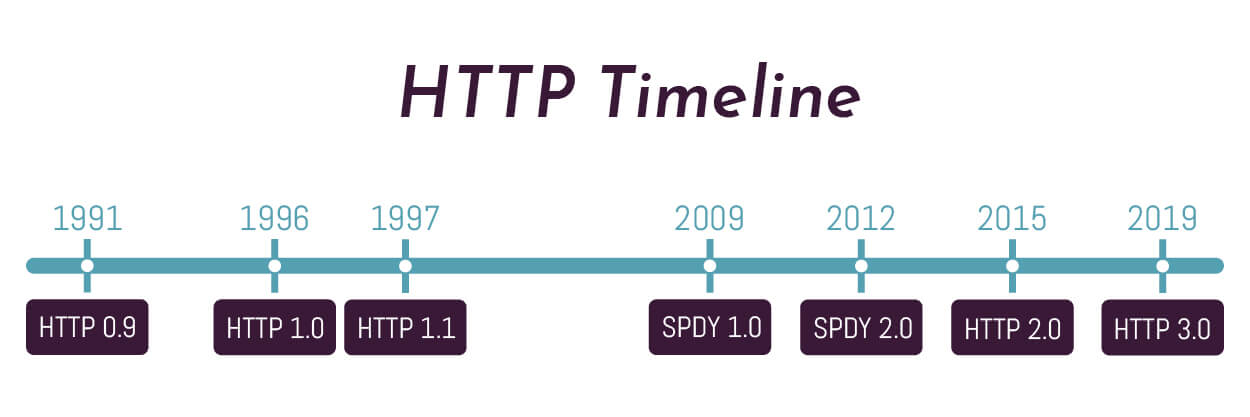
\includegraphics[width=1\textwidth]{http/http_timeline.jpg}
    \caption{HTTP 时间轴}
\end{figure}


\notebox{HTTP标准并未规定TCP就是唯一的传输协议。}


\section{HTTP历史}

\subsection{HTTP/0.9}

\begin{itemize}
    \item 基于TCP协议
    \item 单行请求  GET \qquad 要请求的文档的路径 \qquad  回车符(CRLF)结尾
    \item 连接在文档传输完毕后断开 
\end{itemize}


\subsubsection{重现0.9时代}

\begin{lstlisting}[style=cshell]
    telnet 192.168.31.59 80         # 命令

    Trying 192.168.31.59...
    Connected to 192.168.31.59.

    GET /index.html                 # 命令

    output something... 

    Connection closed by foreign host.
\end{lstlisting}


\begin{figure}[H]
    \centering
    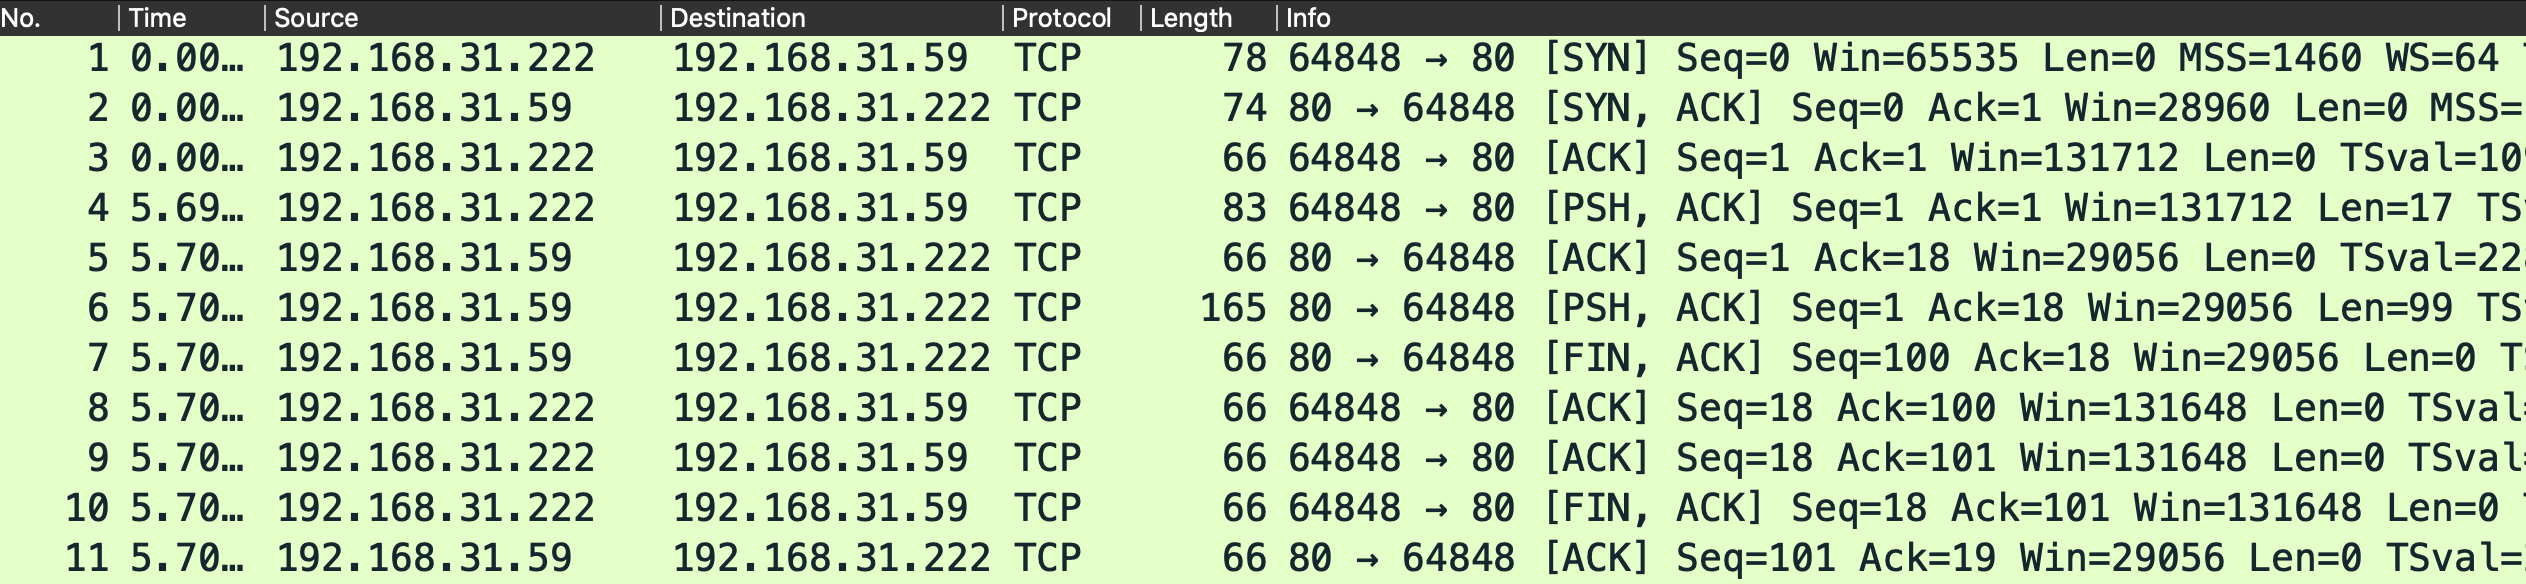
\includegraphics[width=1\textwidth]{http/telnet_http_0_9.png}
    \caption{HTTP/0.9 TCP}
\end{figure}


\begin{figure}[H]
    \centering
    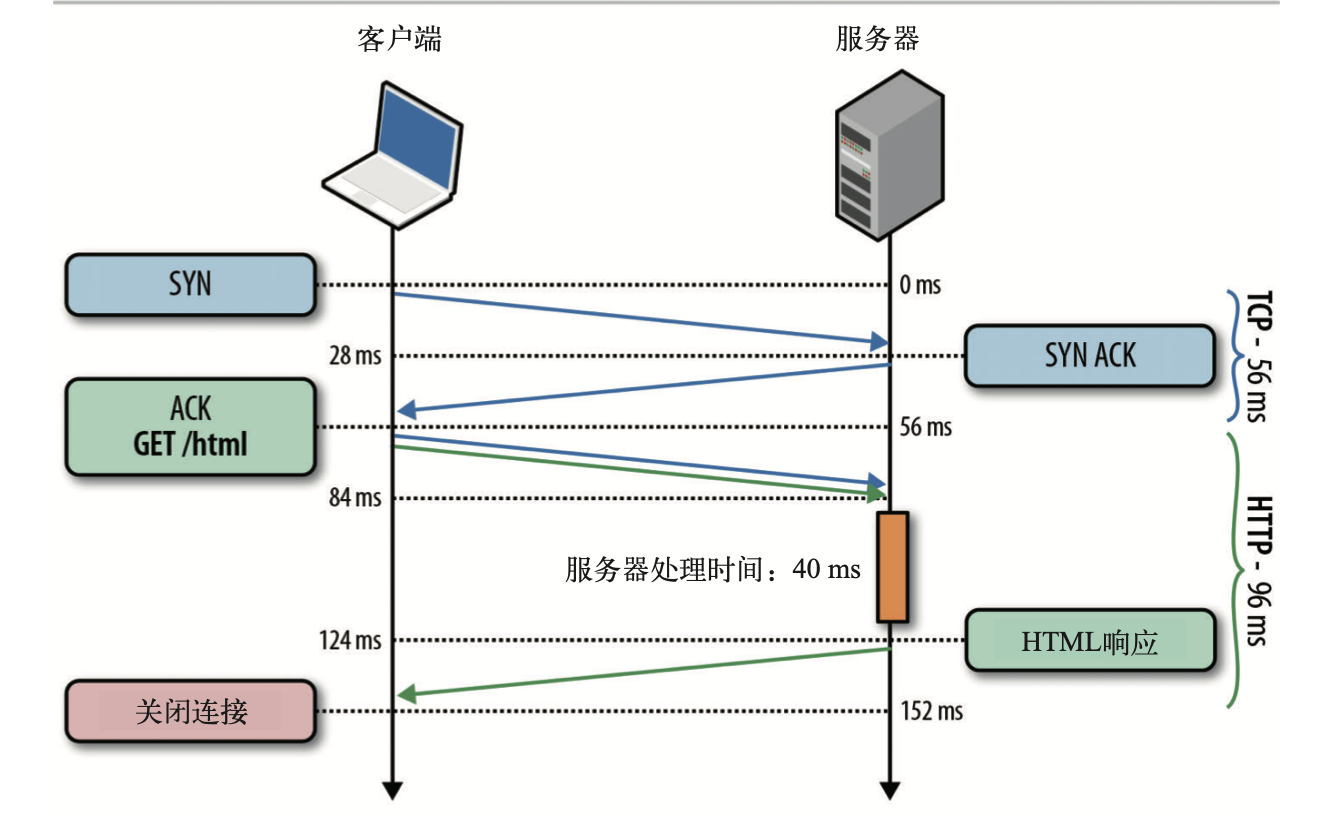
\includegraphics[width=1\textwidth]{http/tcp_http_0_9_flow.png}
    \caption{HTTP/0.9 TCP请求流程图}
\end{figure}





\subsection{HTTP/1.0}

\begin{itemize}
    \item  由起始行、首部、主体构成的请求和响应报文
    \item 响应对象不局限于超文本
    \item 服务器与客户端之间的连接在每次请求之后默认都会关闭
    \item 等等......
\end{itemize}

HTTP/1.0中反向移植了HTTP/1.1持久化连接,通过采用\menlo{Connection: Keep-Alive}可选首部参数。


\subsubsection{重现1.0时代}

\begin{lstlisting}[style=cshell]
    telnet 192.168.31.59 80     # 命令

    Trying 192.168.31.59...
    Connected to 192.168.31.59.

    GET /index.html HTTP/1.0            # 命令
    User-Agent: This is from telnet     # 命令

    HTTP/1.0 200 OK
    Server: nginx/1.10.3 (Ubuntu)
    Date: Thu, 02 Jul 2020 16:36:07 GMT
    Content-Type: text/html
    Content-Length: 99
    Last-Modified: Thu, 02 Jul 2020 16:06:47 GMT
    Connection: close
    ETag: "5efe0617-63"
    Accept-Ranges: bytes

    output something... 

    Connection closed by foreign host.
\end{lstlisting}


\section{HTTP/1.1}

\begin{itemize}
    \item ...... 
    \item 持久连接    persistent connection
    \item 管道化连接   pipeline connection
\end{itemize}


\subsection{持久连接}

* \textbf{在事务处理结束之后仍然保持在打开状态的TCP}

重用对目标服务器打开的空闲持久连接,就可以避免缓慢的连接建立阶段。而且已经打开的连接还可以避免慢启动的拥塞适用阶段。

HTTP/1.1 持久化连接在默认情况下激活的,除非特别指定,否则所有HTTP/1.1所有的连接都是持久化的。如果想要关闭连接需要添加 \menlo{Connection: close}

\begin{figure}[H]
    \centering
    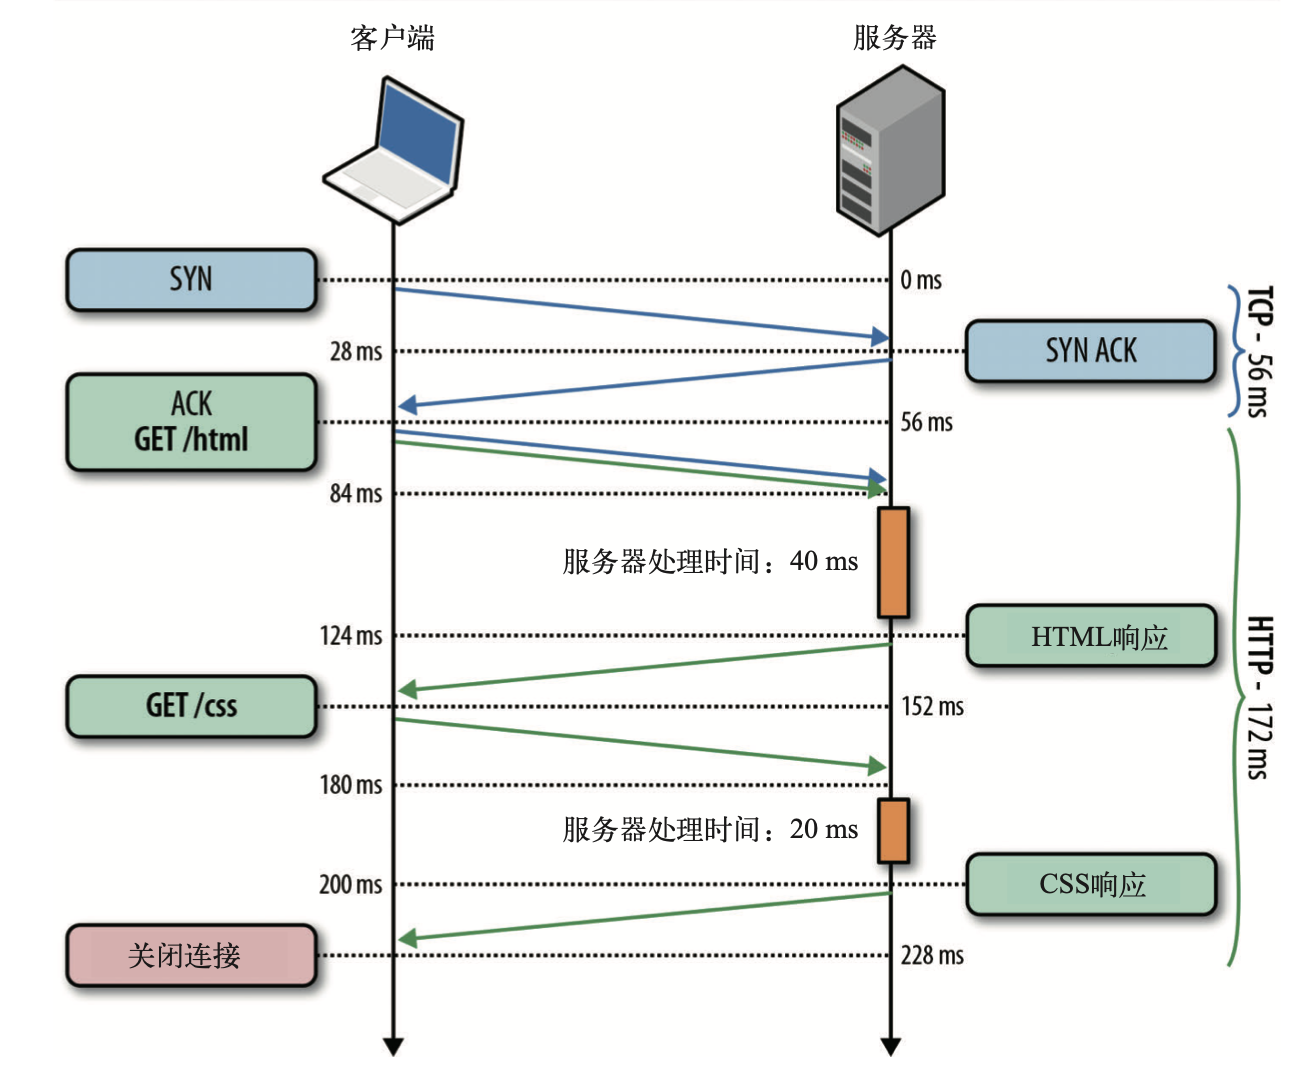
\includegraphics[width=1\textwidth]{http/tcp_http_1_1_persistent_flow.png}
    \caption{HTTP/1.1持久化 TCP请求流程图}
\end{figure}


但是我们的请求还是必须严格按照先进先出(FIFO)的队列顺序:发送请求,等待响应完成,再发送客户端队列中的下一个请求。


\subsection{管道化连接}

\textbf{通过共享的TCP连接发起并发的HTTP请求}

管道化连接是在持久连接的基础上进行的,算是对持久化的优化。把客户端的FIFO队列(请求队列)迁移到服务器(响应队列)。


\begin{figure}[H]
    \centering
    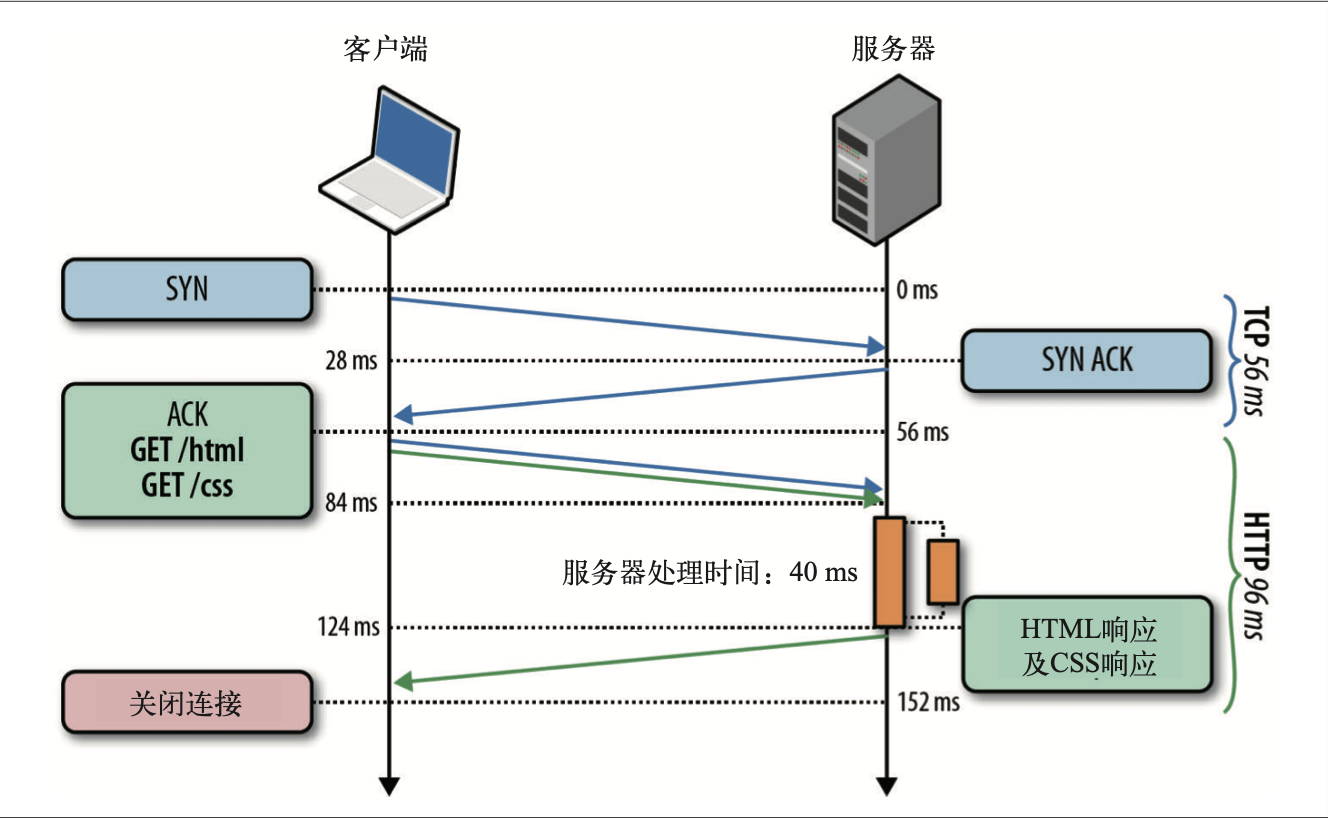
\includegraphics[width=1\textwidth]{http/tcp_http_pipelimne_flow.png}
    \caption{HTTP/1.1持久化 TCP请求流程图}
\end{figure}

严格串行响应,必须按照与请求相同的顺序回送HTTP响应,不支持交错到达(多路复用)

\qquad    HTTP报文中没有序列号标签,如果响应失序了,就没办法与请求匹配了。


按序交付就会导致队首阻塞问题,不能充分利用网络连接,而且会造成服务器缓冲开销等等。

不应该用管道的方式发送非幂等请求

\qquad   例如一系列POST请求,出错的时候我们无法确定那些被正确执行。


目前大部分浏览器是禁用管道技术的。





\subsection{web优化}

并行连接;浏览器默认开启6-8个TCP连接

压缩

缓存

......


\section{HTTP/2}


SPDY(speedy) 是 HTTP 2.0 的基础。

HTTP/2 要解决的问题:

提升性能;

解决HTTP中的“队首阻塞”问题;

并行操作无需与服务器建立多个连接,改进TCP的利用率,尤其是拥塞控制方面;

兼容HTTP/1.1的语义;



\begin{itemize}
    \item One TCP connection
    \item Binary framing layer
    \item Streams and Multiplexing
    \item Header compression (HPACK)
\end{itemize}


\textbf{HTTP/2直观感受}


\href{https://http2.golang.org/gophertiles}{A grid of 180 tiled images is below. Compare}

\subsection{Connection}


\begin{itemize}
    \item   TCP连接三次握手 
    \item   TCP慢启动拥塞控制
    \item   用户捎带确认的TCP延迟确认算法
    \item   TIME\_WAIT时延和端口耗尽
\end{itemize}


HTTP/2两个标识符

\begin{itemize}
    \item h2c
    \item h2
\end{itemize}  

\textbf{h2c}

表示HTTP/2协议运行在明文TCP上。

标识通过明文 TCP 运行 HTTP/2 的协议。此标识符用于 HTTP/1.1 升级标头字段以及标识 HTTP/2 over TCP 的任何位置。

\textbf{h2}

表示 HTTP/2 使用传输层安全性(TLS)TLS的协议。用于 TLS 应用层协议协商(ALPN)。


\subsubsection{通过HTTP Uri启动连接}

发起请求


\begin{lstlisting}[style=cshell]

    GET /index.html HTTP/1.1
    host: nghttp2.org
    connection: Upgrade, HTTP2-Settings
    upgrade: h2c
    http2-settings: AAMAAABkAAQAAP__

\end{lstlisting}


如果不支持HTTP/2,服务忽略h2c 首部字段,返回一个不包含升级的首部响应。

\begin{lstlisting}[style=cshell]

    HTTP/1.1 200 OK
    ...

\end{lstlisting}


如果服务端支持HTTP/2则返回101协议来接受升级请求。101协议响应结束后,服务端开始发送包含HTTP/2帧的请求,第一个被服务端发送的帧是设置帧。
客户端在收到101协议响应后,也发送一个包含设置帧的请求。

\begin{lstlisting}[style=cshell]

HTTP/1.1 101 Switching Protocols
Connection: Upgrade
Upgrade: h2c

\end{lstlisting}


\begin{figure}[H]
    \centering
    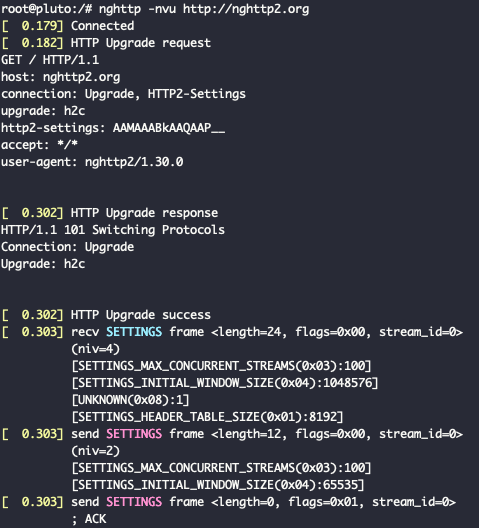
\includegraphics[width=1\textwidth]{http/nghttp_client_http_upgrade.png}
    \caption{nghttp模拟HTTP/1.1 Upgrade}
\end{figure}


\subsubsection{通过HTTPS Uri启动连接}

ALPN(应用层协议协商)

\begin{figure}[H]
    \centering
    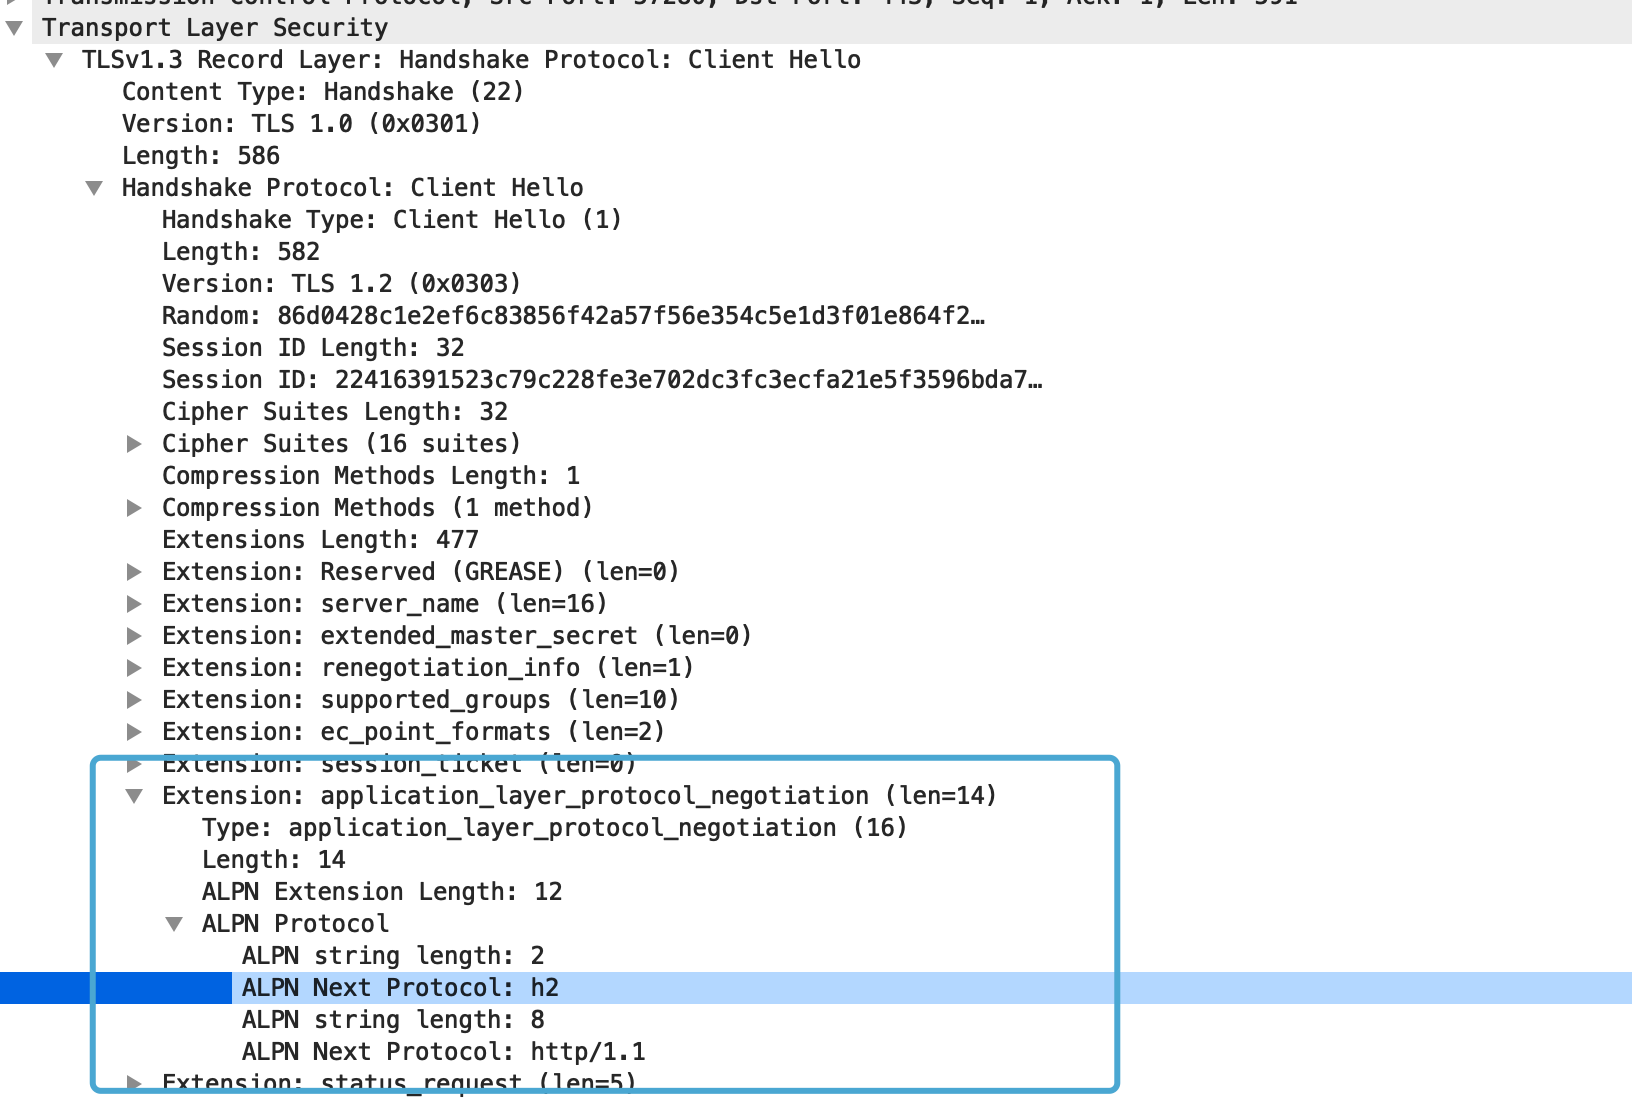
\includegraphics[width=1\textwidth]{http/http_2_client_alpn.png}
    \caption{客户端发起Client Hello协议}
\end{figure}


\begin{figure}[H]
    \centering
    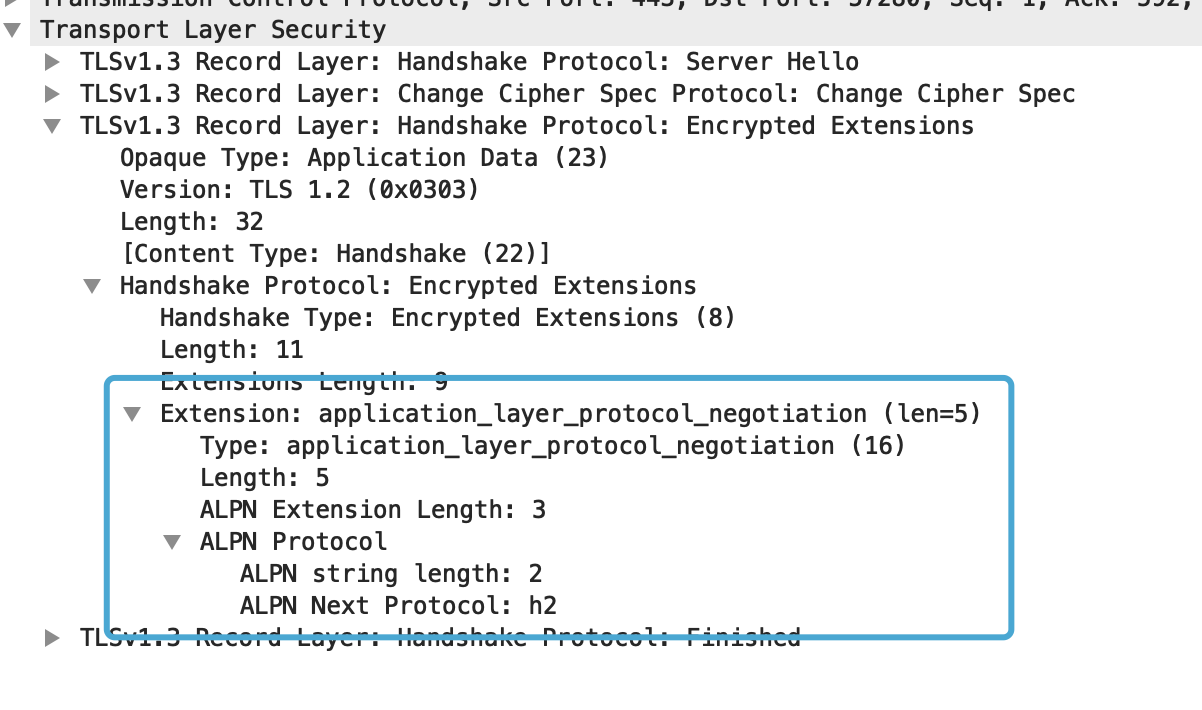
\includegraphics[width=1\textwidth]{http/http_2_server_alpn.png}
    \caption{服务端发起Server Hello协议}
\end{figure}


\subsubsection{HTTP/2 Connection Preface}


在 HTTP/2 中,每个端点都需要发送连接前奏作为正在使用的协议的最终确认,并建立 HTTP/2 连接的初始设置。客户端和服务器各自发送不同的连接前奏。

客户端连接前奏以 24 个八位字节的序列开始,以十六进制表示法为:

\begin{lstlisting}[style=cshell]


0x505249202a20485454502f322e300d0a0d0a534d0d0a0d0a

# 字符串格式: PRI * HTTP/2.0\r\n\r\nSM\r\n\r\n

\end{lstlisting}

该序列必须后跟 可为空的SETTINGS 帧。


服务器连接前奏包含一个可为空的 SETTINGS 帧,该帧必须是服务器在 HTTP/2 连接中发送的第一帧。

服务器可以在客户端发送附加帧之前发送 SETTINGS,从而提供避免此问题的机会。



\begin{figure}[H]
    \centering
    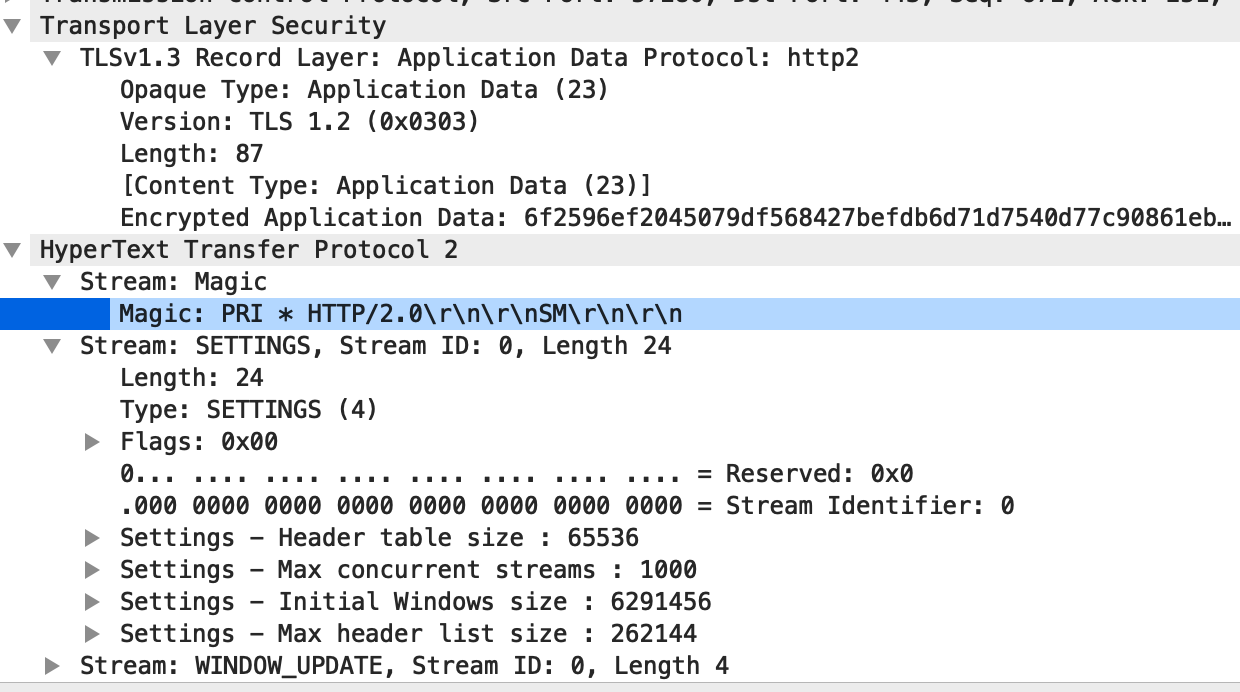
\includegraphics[width=1\textwidth]{http/http_2_connection_preface_prism.png}
    \caption{Connection Preface prism}
\end{figure}


\subsection{Frames}


\begin{figure}[H]
    \centering
    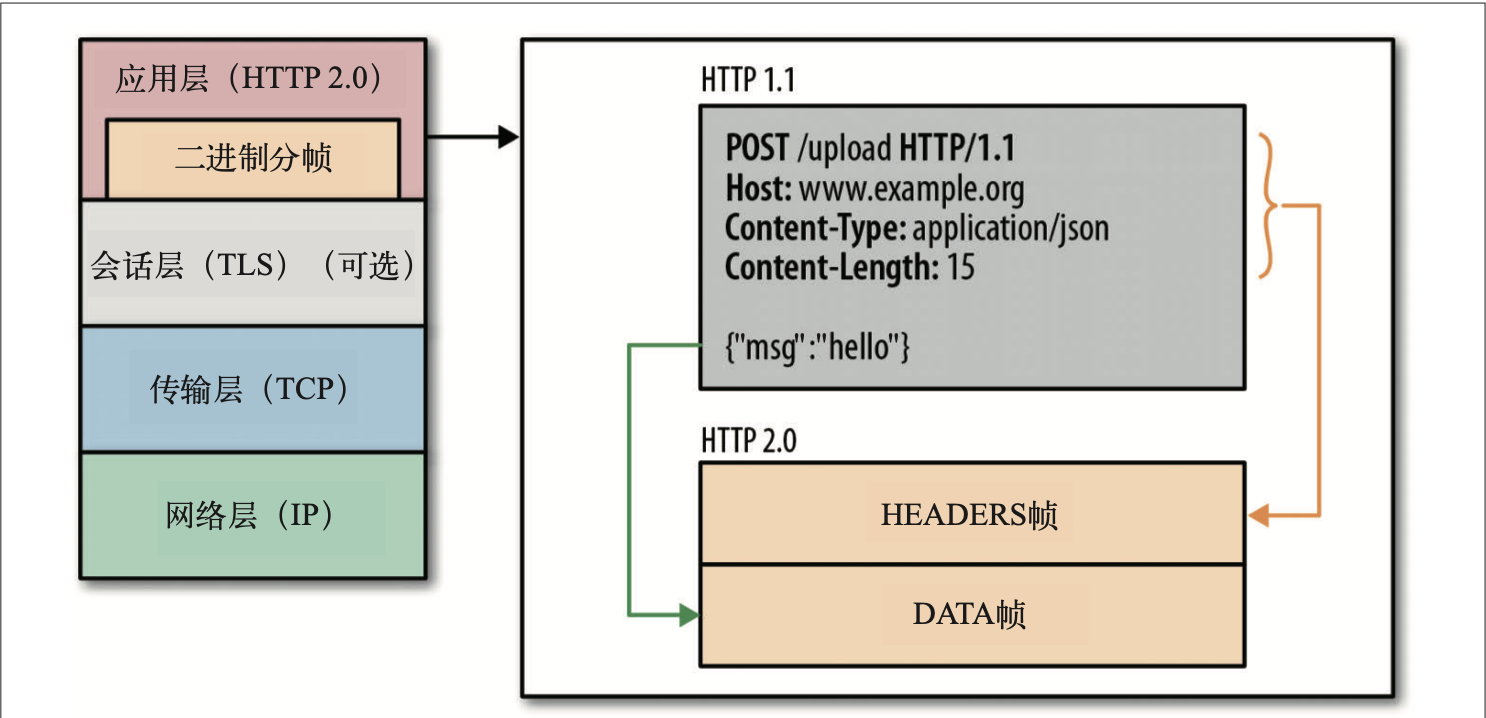
\includegraphics[width=1\textwidth]{http/binary_framing_layer.png}
    \caption{二进制分帧层}
\end{figure}


所有 HTTP 2.0 通信都在一个连接上完成,这个连接可以承载任意数量的双向数据流。
相应地,每个数据流以消息的形式发送,而消息由一或多个帧组成,这些帧可以乱序发送,然后再根据每个帧首部的流标识符重新组装。

HTTP 2.0 的二进制分帧机制解决了 HTTP 1.x 中存在的队首阻塞问题。

\subsubsection{Frame Layout}

帧就是HTTP 2.0 通信的最小单位,每个帧包含帧首部,至少也会标识出当前帧所属的流。

\begin{figure}[H]
    \centering
    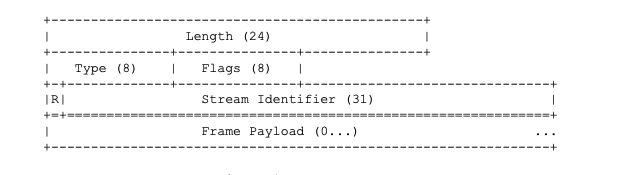
\includegraphics[width=1\textwidth]{http/frame_layout.png}
    \caption{HTTP/2帧结构}
\end{figure}


\begin{table}[H]
    \renewcommand{\arraystretch}{2}
    \centering
    \begin{tabular} {p{70pt}p{50pt}p{250pt}}
    \hline
    名称                 & 长度      &   描述                                      \\ \hline
    Length              & 3字节     &   表示帧负载的长度(取值范围为$2^{14}$ $\sim$ $2^{24}$-1)。默认最大帧大小是$2^{14}$。可以通过SETTINGS帧修改。            \\ \hline
    Type                & 1字节     &   当前帧类型                                  \\ \hline
    Flags               & 1字节     &   具体帧类型的标识                            \\ \hline
    R                   & 1位       &   保留位                                    \\ \hline
    Stream Identifier    & 31位      &   每个流的唯一ID                             \\ \hline
    Frame Payload       & 长度可变   &   真实帧内容;长度设置在Length中               \\ \hline
    \end{tabular}
    \caption{\label{tab:table-name}帧字段}
    \end{table}


    前9个字节是帧的固定结构。解析时只需要读取这些字节。



\begin{table}[H]
    \renewcommand{\arraystretch}{1.5}
    \centering
     \begin{tabular} {p{100pt}p{30pt}p{250pt}}
     \hline
    名称             & ID      &   描述                             \\ \hline
    DATA            & 0x0     &   流核心内容                          \\ \hline
    HEADERS         & 0x1     &  HTTP首部以及可选的优先级参数           \\ \hline
    PRIORITY        & 0x2     &  指示或者更改流的优先级和依赖           \\ \hline
    RST\_STREAM     & 0x3     &  允许一段停止流(通常由于错误导致的)     \\ \hline
    SETTINGS        & 0x4     &  协商连接级参数                       \\ \hline
    PUSH\_PROMISE   & 0x5     &  提示客户端,服务器要推送东西            \\ \hline
    PING            & 0x6     &  测试连接可用性和往返时延(RTT)           \\ \hline
    GOAWAY          & 0x7     &  告诉另一段,当前端已结束                \\ \hline
    WINDOW\_UPDATE  & 0x8     &  用于流量控制;协商一段将要接受多少字节     \\ \hline
    CONTINUATION    & 0x9     &  用以扩展HEADER数据块                   \\ \hline
    \end{tabular}
    \caption{\label{tab:table-name}帧类型}
    \end{table}


\subsubsection{DATA}

\begin{figure}[H]
    \centering
    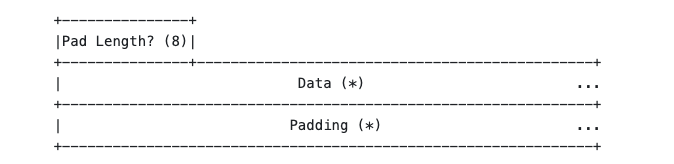
\includegraphics[width=1\textwidth]{http/data_frame_payload.png}
    \caption{DATA帧结构}
\end{figure}

DATA 帧包含以下几个字段:

Pad Length:
一个 8 位字段,包含以八位字节为单位的帧填充长度。该字段是有条件的,仅在设置了 PADDED 标志时才存在。

Data:
应用数据。在减去存在的其他字段的长度之后,data 的大小是帧有效载荷的剩余部分。

Padding:
填充的八位字节,它不包含应用程序语义值。发送时,填充的八位字必须设置为零。接收方没有义务验证填充,但可以将非零填充视为 PROTOCOL\_ERROR 类型的连接错误。


DATA 帧定义了以下 flag 标识:

END\_STREAM (0x1):
设置这个字段的时候,位 0 表示该帧是端点为将要发送的标识流的最后一帧。设置此标志会导致流进入"半关闭"状态或者"关闭"状态。

PADDED (0x8):
设置这个字段的时候,位 3 表示存在 Pad Length 字段及其描述的任何填充。


\begin{figure}[H]
    \centering
    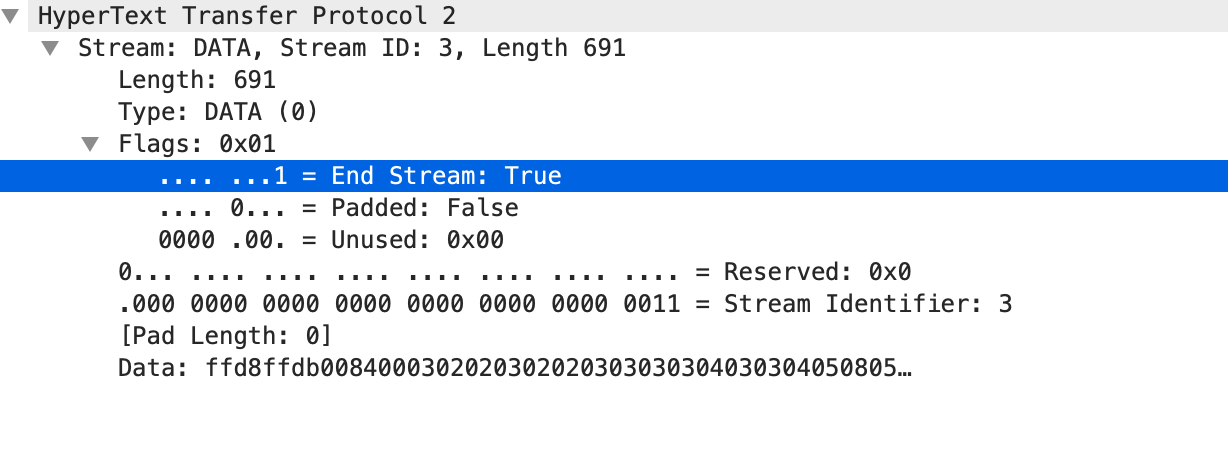
\includegraphics[width=1\textwidth]{http/data_frame_end_stream_flags.png}
    \caption{END\_STREAM}
\end{figure}



DATA 帧必须与某一个流相互关联。如果接收到其流标识符字段为 0x0 的 DATA 帧,则接收方必须以 PROTOCOL\_ERROR 类型的连接错误进行响应。

DATA 帧会受到流量控制,只能在流处于“打开”或“半关闭(远程)”状态时发送。整个 DATA 帧有效载荷包含在流量控制中,包括 Pad Length 和 Padding 字段(如果存在)。如果收到的数据帧的流不是“打开”或“半关闭(本地)”状态,则接收方必须以 STREAM\_CLOSED 类型的流错误进行响应。

填充八位字节的总数由填充长度字段的值确定。如果填充的长度是帧有效负载的长度或更长,则接收方必须将其视为 PROTOCOL\_ERROR 类型的连接错误。


\subsubsection{HEADERS}

\begin{figure}[H]
    \centering
    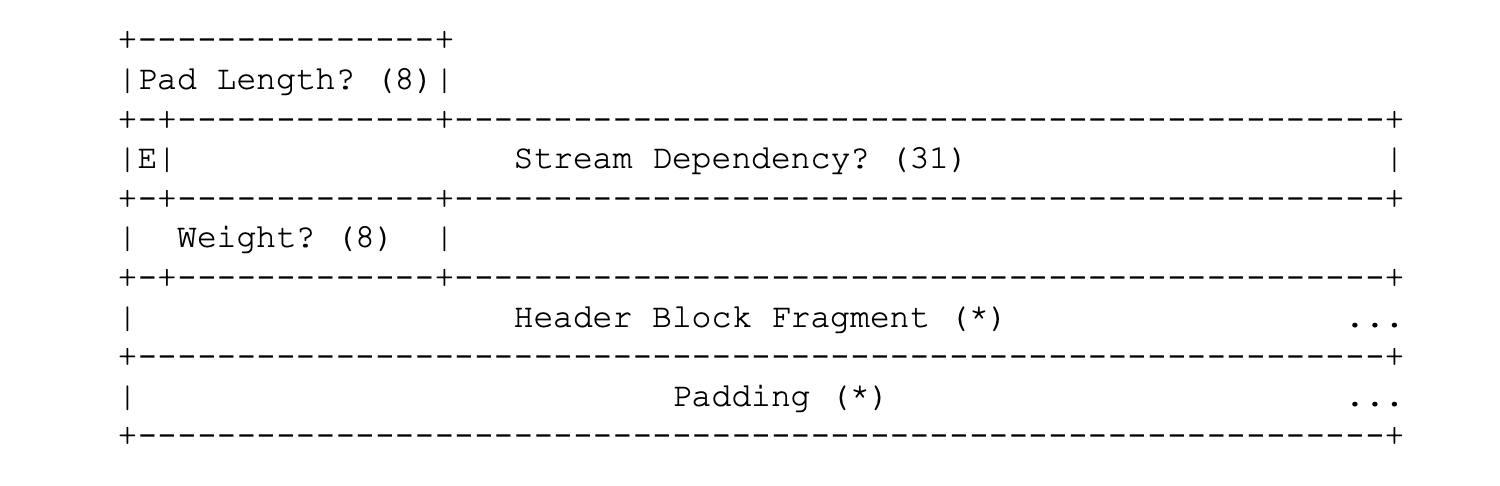
\includegraphics[width=1\textwidth]{http/headers_frame_payload.png}
    \caption{HEADERS帧结构}
\end{figure}


Pad Length: 指定 Padding 长度,存在则代表 PADDING flag 被设置

E: 一个比特位声明流的依赖性是否是排他的,存在则代表 PRIORITY flag 被设置

Stream Dependency: 指定一个 stream identifier,代表当前流所依赖的流的 id,存在则代表 PRIORITY flag 被设置

Weight: 一个无符号 8 为整数,代表当前流的优先级权重值 (1~256),存在则代表 PRIORITY flag 被设置

Header Block Fragment: header 块片段

Padding: 填充字节,没有具体语义,作用与 DATA 的 Padding 一样,存在则代表 PADDING flag 被设置

HEADERS 帧有以下标识 (flags):

END\_STREAM: bit 0 设为 1 代表当前 header 块是发送的最后一块,但是带有 END\_STREAM 标识的 HEADERS 帧后面还可以跟 CONTINUATION 帧 (这里可以把 CONTINUATION 看作 HEADERS 的一部分)

END\_HEADERS: bit 2 设为 1 代表 header 块结束

PADDED: bit 3 设为 1 代表 Pad 被设置,存在 Pad Length 和 Padding

PRIORITY: bit 5 设为 1 表示存在 Exclusive Flag (E), Stream Dependency, 和 Weight


\begin{figure}[H]
    \centering
    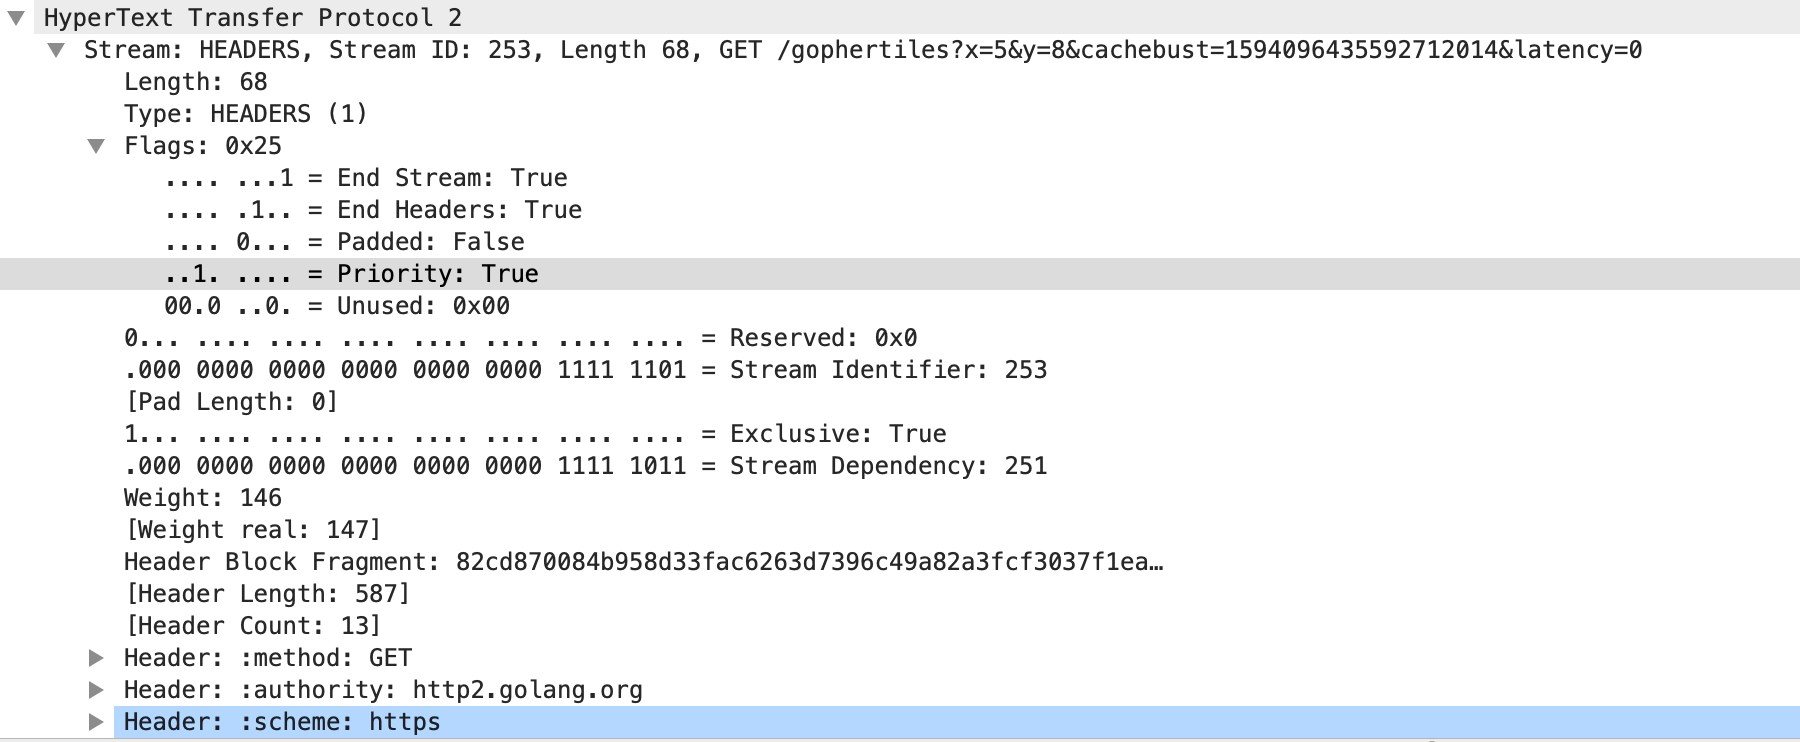
\includegraphics[width=1\textwidth]{http/http_2_headers_frame_flags.png}
    \caption{HEADERS帧结构}
\end{figure}



\subsubsection{SETTINGS}

\begin{figure}[H]
    \centering
    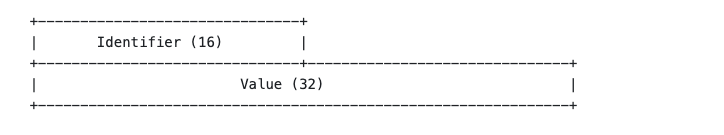
\includegraphics[width=1\textwidth]{http/http_2_setting_format.png}
    \caption{SETTINGS帧结构}
\end{figure}

SETTINGS\_HEADER\_TABLE\_SIZE(0x1)

SETTINGS\_ENABLE\_PUSH(0x2)

SETTINGS\_MAX\_CONCURRENT\_STREAMS(0x3)

SETTINGS\_INITIAL\_WINDOW\_SIZE(0x4)

SETTINGS\_MAX\_FRAME\_SIZE(0x5)

SETTINGS\_MAX\_HEADER\_LIST\_SIZE(0x6)


\subsection{Stream}

HTTP/2连接上独立的,双向的帧序列交换。

\begin{figure}[H]
    \centering
    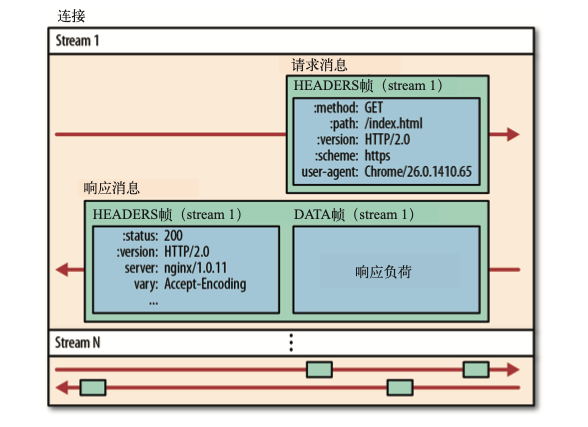
\includegraphics[width=1\textwidth]{http/http_2_frame.png}
    \caption{流、消息和帧}
\end{figure}

客户端到服务端的h2连接建立之后,通过发送HEADERS帧来启动新的流,如果首部需要跨多个帧,可能还会发送CONTINUATION帧。
后续流启动会发送一个带有自增Stream Identifier的新HEADERS帧。

\notebox{HEADERS和CONTINUATION帧必须是有序的。}


stream 流使用无符号的 31 位整数标识。
由客户端发起的流必须使用奇数编号的流标识符。

服务器发起的必须使用偶数编号的流标识符。

流标识符零(0x0)用于连接控制消息;零流标识符不能用于建立新的 stream 流。

HTTP/1.1 Upgrade to HTTP/2 时响应的流 ID 是 0x1,在升级完成之后,流 0x1 在客户端会转为 half-closed (local) 状态,因此这种情况下客户端不能用 0x1 初始化一个流。
因为HTTP/1.1请求已经完成了。


\subsubsection{流生命周期}

\begin{figure}[H]
    \centering
    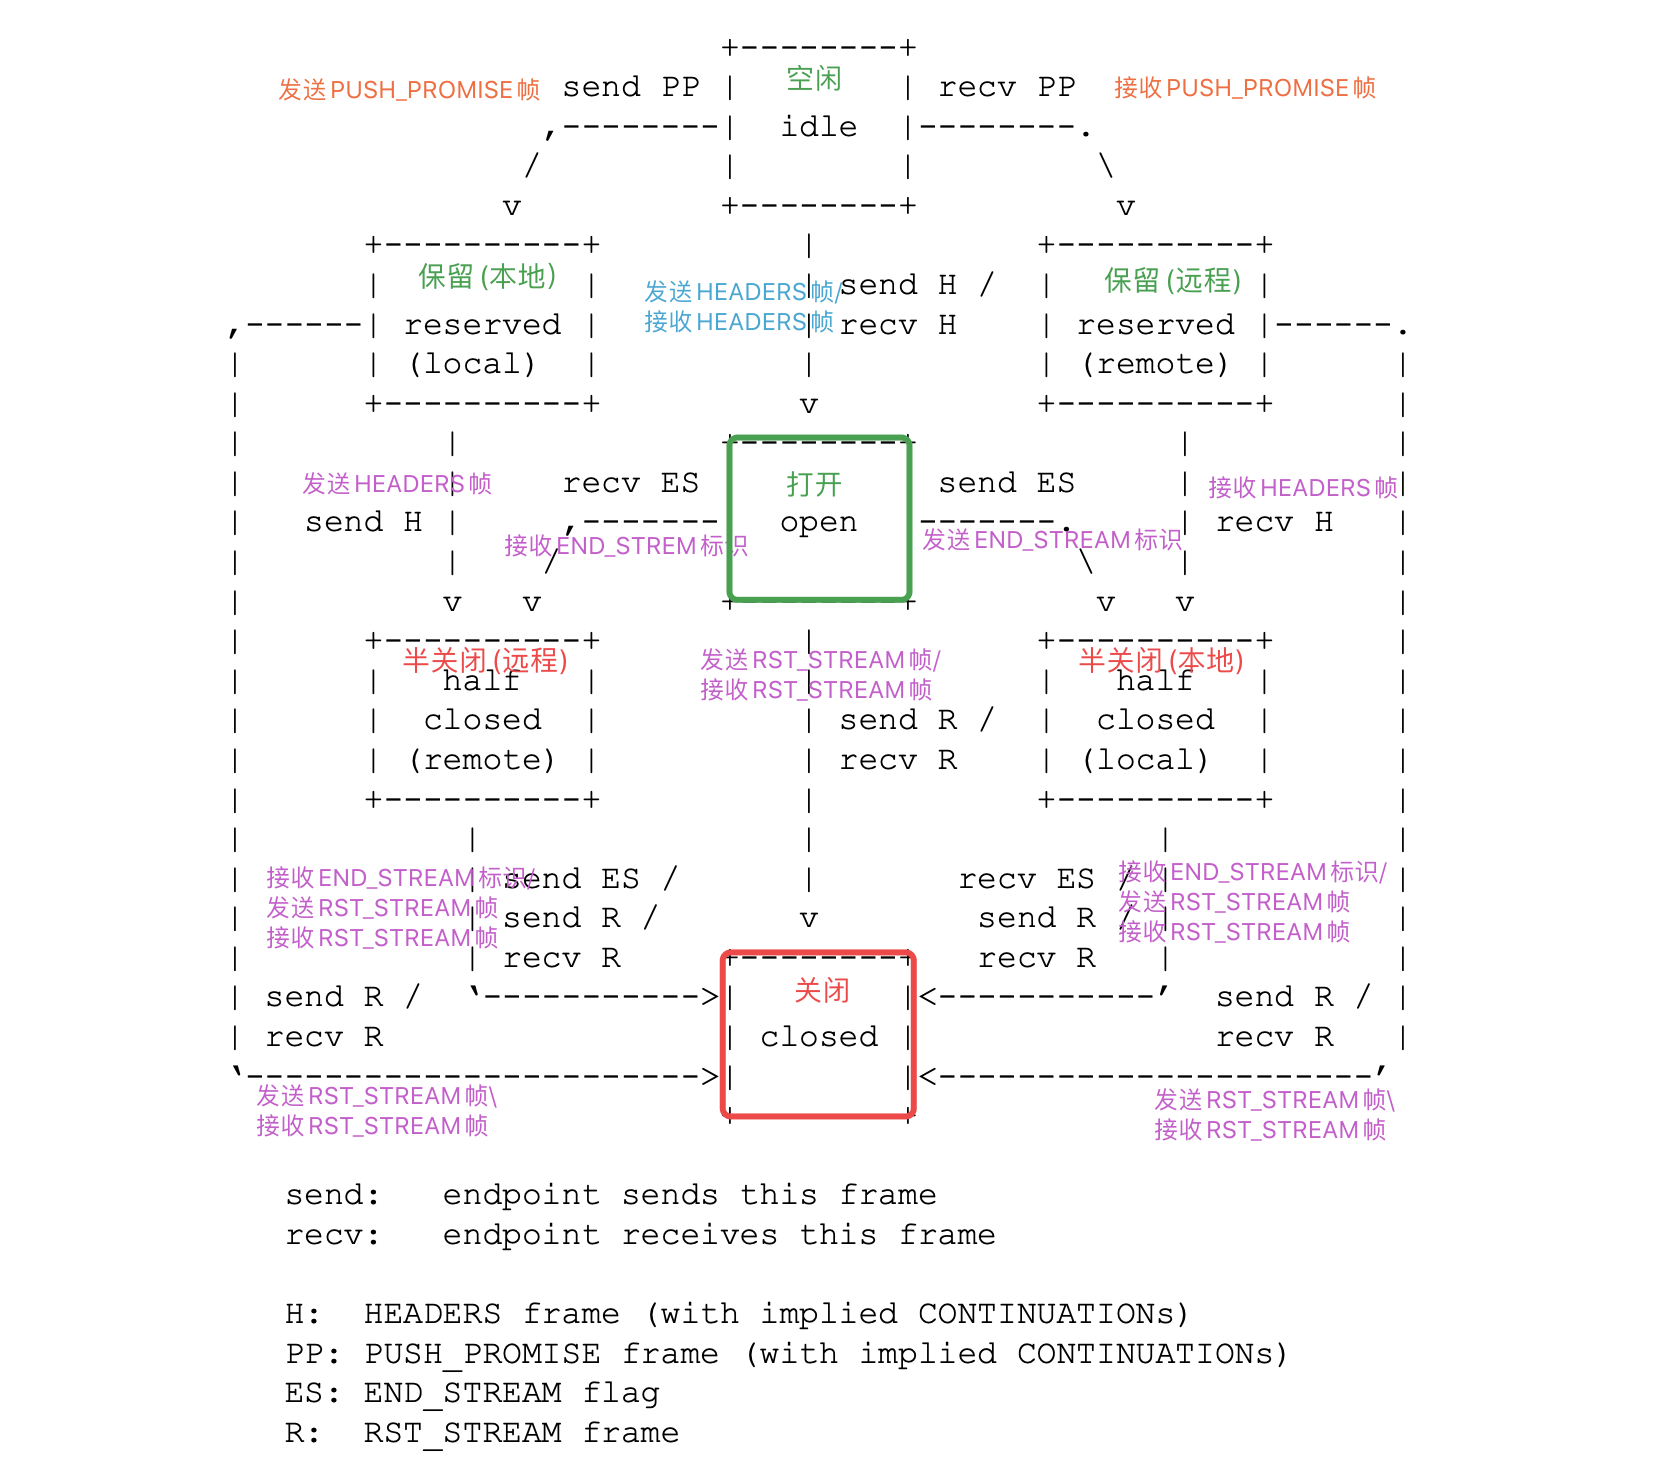
\includegraphics[width=1\textwidth]{http/stream_life.png}
    \caption{流生命周期}
\end{figure}


\textbf{idle}

所有的 stream 流都是从空闲态开始的。

\textbf{reserved}

reserved,为推送保留一个流稍后使用。

reserved(local)

\qquad 服务器端发送完PUSH\_PROMISE帧本地预留的一个用于推送流所处于的状态

\qquad 只能发送HEADERS、RST\_STREAM、PRIORITY帧

\qquad 只能接收RST\_STREAM、PRIORITY、WINDOW\_UPDATE帧

reserved(remote)

\qquad 客户端接收到PUSH\_PROMISE帧,本地预留的一个用于接收推送流所处于的状态

\qquad 只能发送WINDOW\_UPDATE、RST\_STREAM、PRIORITY帧

\qquad 只能接收RST\_STREAM、PRIORITY、HEADERS帧

\qquad 不满足条件,需要报PROTOCOL\_ERROR类型连接错误


\textbf{open}

\qquad 用于两端发送帧,需要发送数据的对等端需要遵守流量控制的通告。

\qquad 每一端可以发送包含END\_STREAM标志位的帧,导致流进入"half closed"状态

\qquad 每一端都可以发送RST\_STREAM帧,流进入"closed"状态


 \textbf{half closed}

 half closed(local)

 发送包含有END\_STREAM标志位帧的一端,流进入本地半关闭状态

 \qquad 不能发送WINDOW\_UPDATE,PRIORITY和RST\_STREAM帧

 \qquad 可以接收到任何类型帧

 \qquad 接收者可以忽略WINDOW\_UPDATE帧,后续可能会马上接收到包含有END\_STREAM标志位帧

 \qquad 接收到优先级PRIORITY帧,可用来变更依赖流的优先级顺序

 \qquad 一旦接收到包含END\_STREAM标志位的帧,将进入"closed"状态

 half closed(remote)
 
接收到包含有END\_STREAM标志位帧的一端,流进入远程半关闭状态
 
    \qquad 对流量控制窗口可不用维护

    \qquad 只能接收RST\_STREAM、PRIORITY、WINDOW\_UPDATE帧,否则报STREAM\_CLOSED流错误

    \qquad 终端可以发送任何类型帧,但需要遵守对端的当前流的流量控制限制

    \qquad 一旦发送包含END\_STREAM标志位的帧,将进入"closed"状态

一旦接收或发送RST\_STREAM帧,流将进入"closed"状态

\textbf{closed}

流的最终关闭状态



\begin{figure}[H]
    \centering
    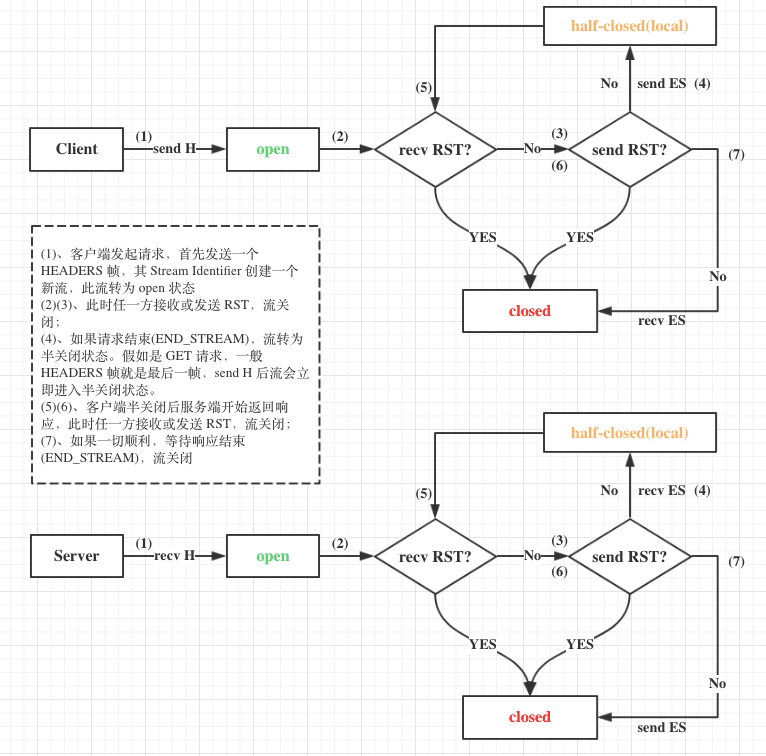
\includegraphics[width=1\textwidth]{http/http_2_request_stream.png}
    \caption{请求/响应流状态态转化}
\end{figure}

\begin{figure}[H]
    \centering
    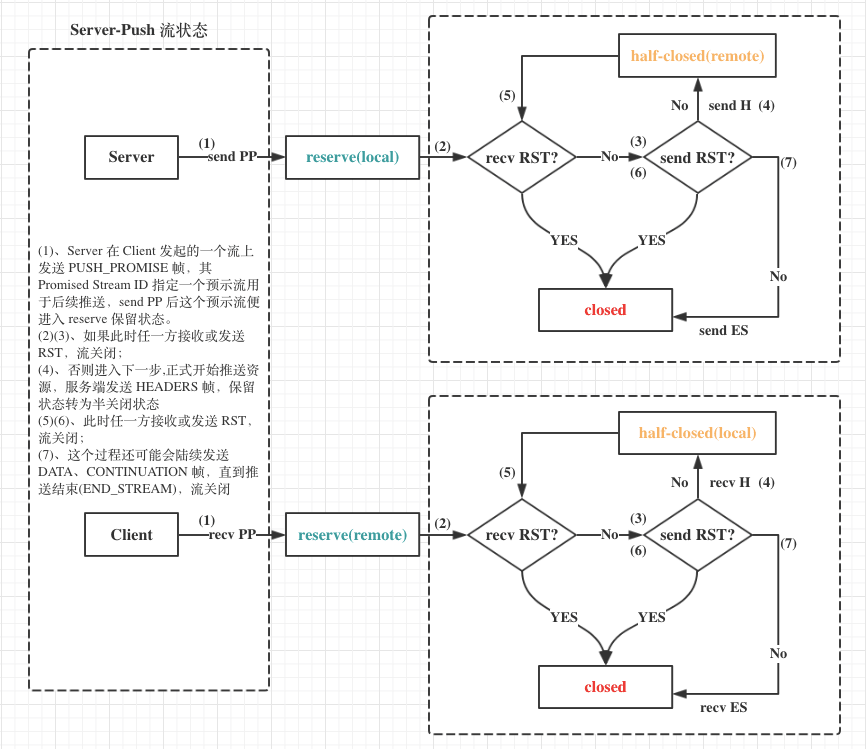
\includegraphics[width=1\textwidth]{http/http_2_server_push.png}
    \caption{Server Push}
\end{figure}


\subsubsection{流优先级}

\begin{itemize}
    \item 依赖关系
    \item 权重
\end{itemize} 


客户端可以通过在打开流的 HEADERS 帧中包含优先级信息来为新的流分配优先级。在任何其他时间,PRIORITY 帧可用于更改流的优先级。

确定优先级的目的是允许端点在管理并发流时表达它希望其对端如何分配资源。最重要的是,当发送容量有限时,可以使用优先级来选择用于发送帧的流。

可以通过将流标记为依赖其他流的完成,来确定流的优先级。为每个依赖项分配一个相对权重,该数字用于确定分配给依赖于相同流的 stream 流的可用资源的相对比例。


\begin{figure}[H]
    \centering
    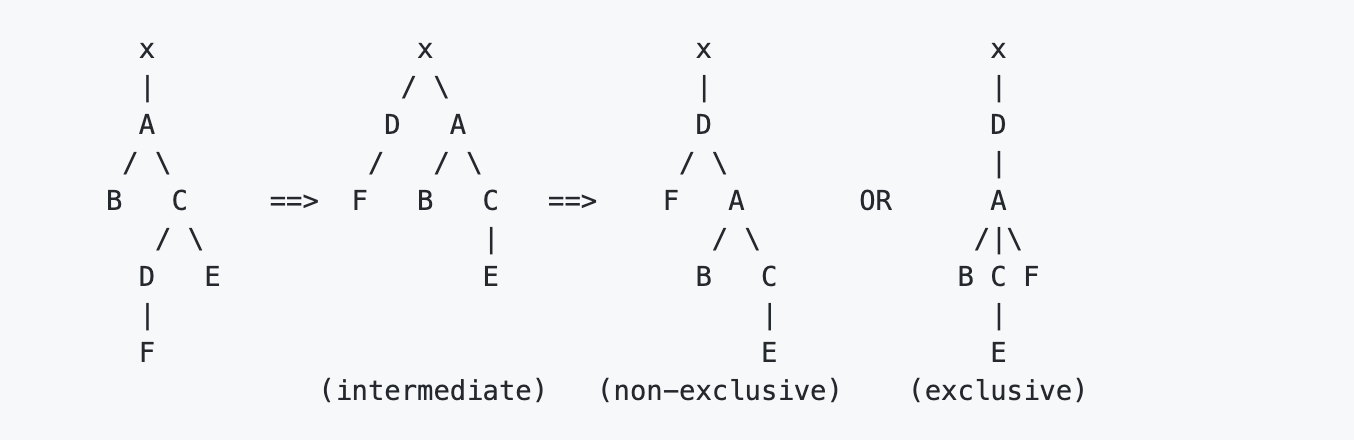
\includegraphics[width=1\textwidth]{http/http_2_dependency_reprioritization.png}
    \caption{依赖优先级调整}
\end{figure}

D 优先级变高


\begin{figure}[H]
    \centering
    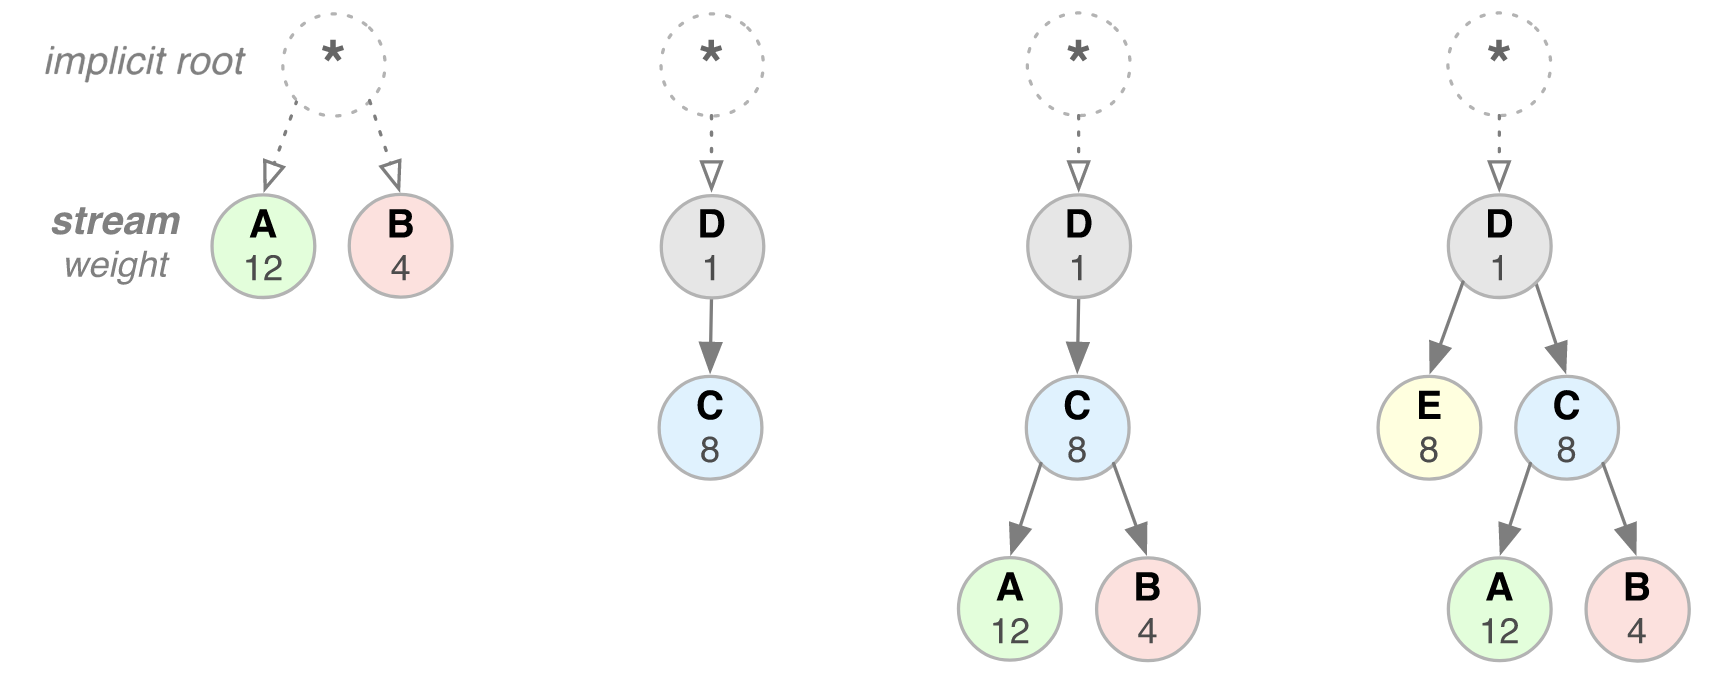
\includegraphics[width=1\textwidth]{http/http_2_dependency_weighting.png}
    \caption{依赖以及权重}
\end{figure}


\subsubsection{流量控制}

HTTP/2 通过使用 WINDOW\_UPDATE 帧提供流量控制

只有 DATA 帧受流量控制

流控制窗口的默认值设为 65,535 字节

\begin{figure}[H]
    \centering
    
\includegraphics[width=1\textwidth]{http/http_2_flow_control_demo.png}
    \caption{流量控制示例}
\end{figure}


\subsubsection{服务器推送}

\href{https://www.nginx.com/blog/nginx-1-13-9-http2-server-push/}{http2-server-push}


\section{HPACK}

\subsection{Deflate}

LZ77 + Huffman

CRIME漏洞

攻击者在请求中(cookie)添加数据,观察压缩加密后的数据量是否会小于预期,如果变小了,注入的文本和请求中的其他内容有重复。


\subsection{Huffman Coding}

\href{https://people.ok.ubc.ca/ylucet/DS/Huffman.html}{动画演示}

\subsection{索引表}

静态表(Static Table)和动态表(Dynamic Table)

\textbf{}{静态表}

静态索引表由预定义的首部字段构成。包含61个预定义Header key-value。

\href{https://tools.ietf.org/html/rfc7541#appendix-A}{静态索引表字段}


\textbf{动态表}

\subsection{实现}

\begin{figure}[H]
    \centering
    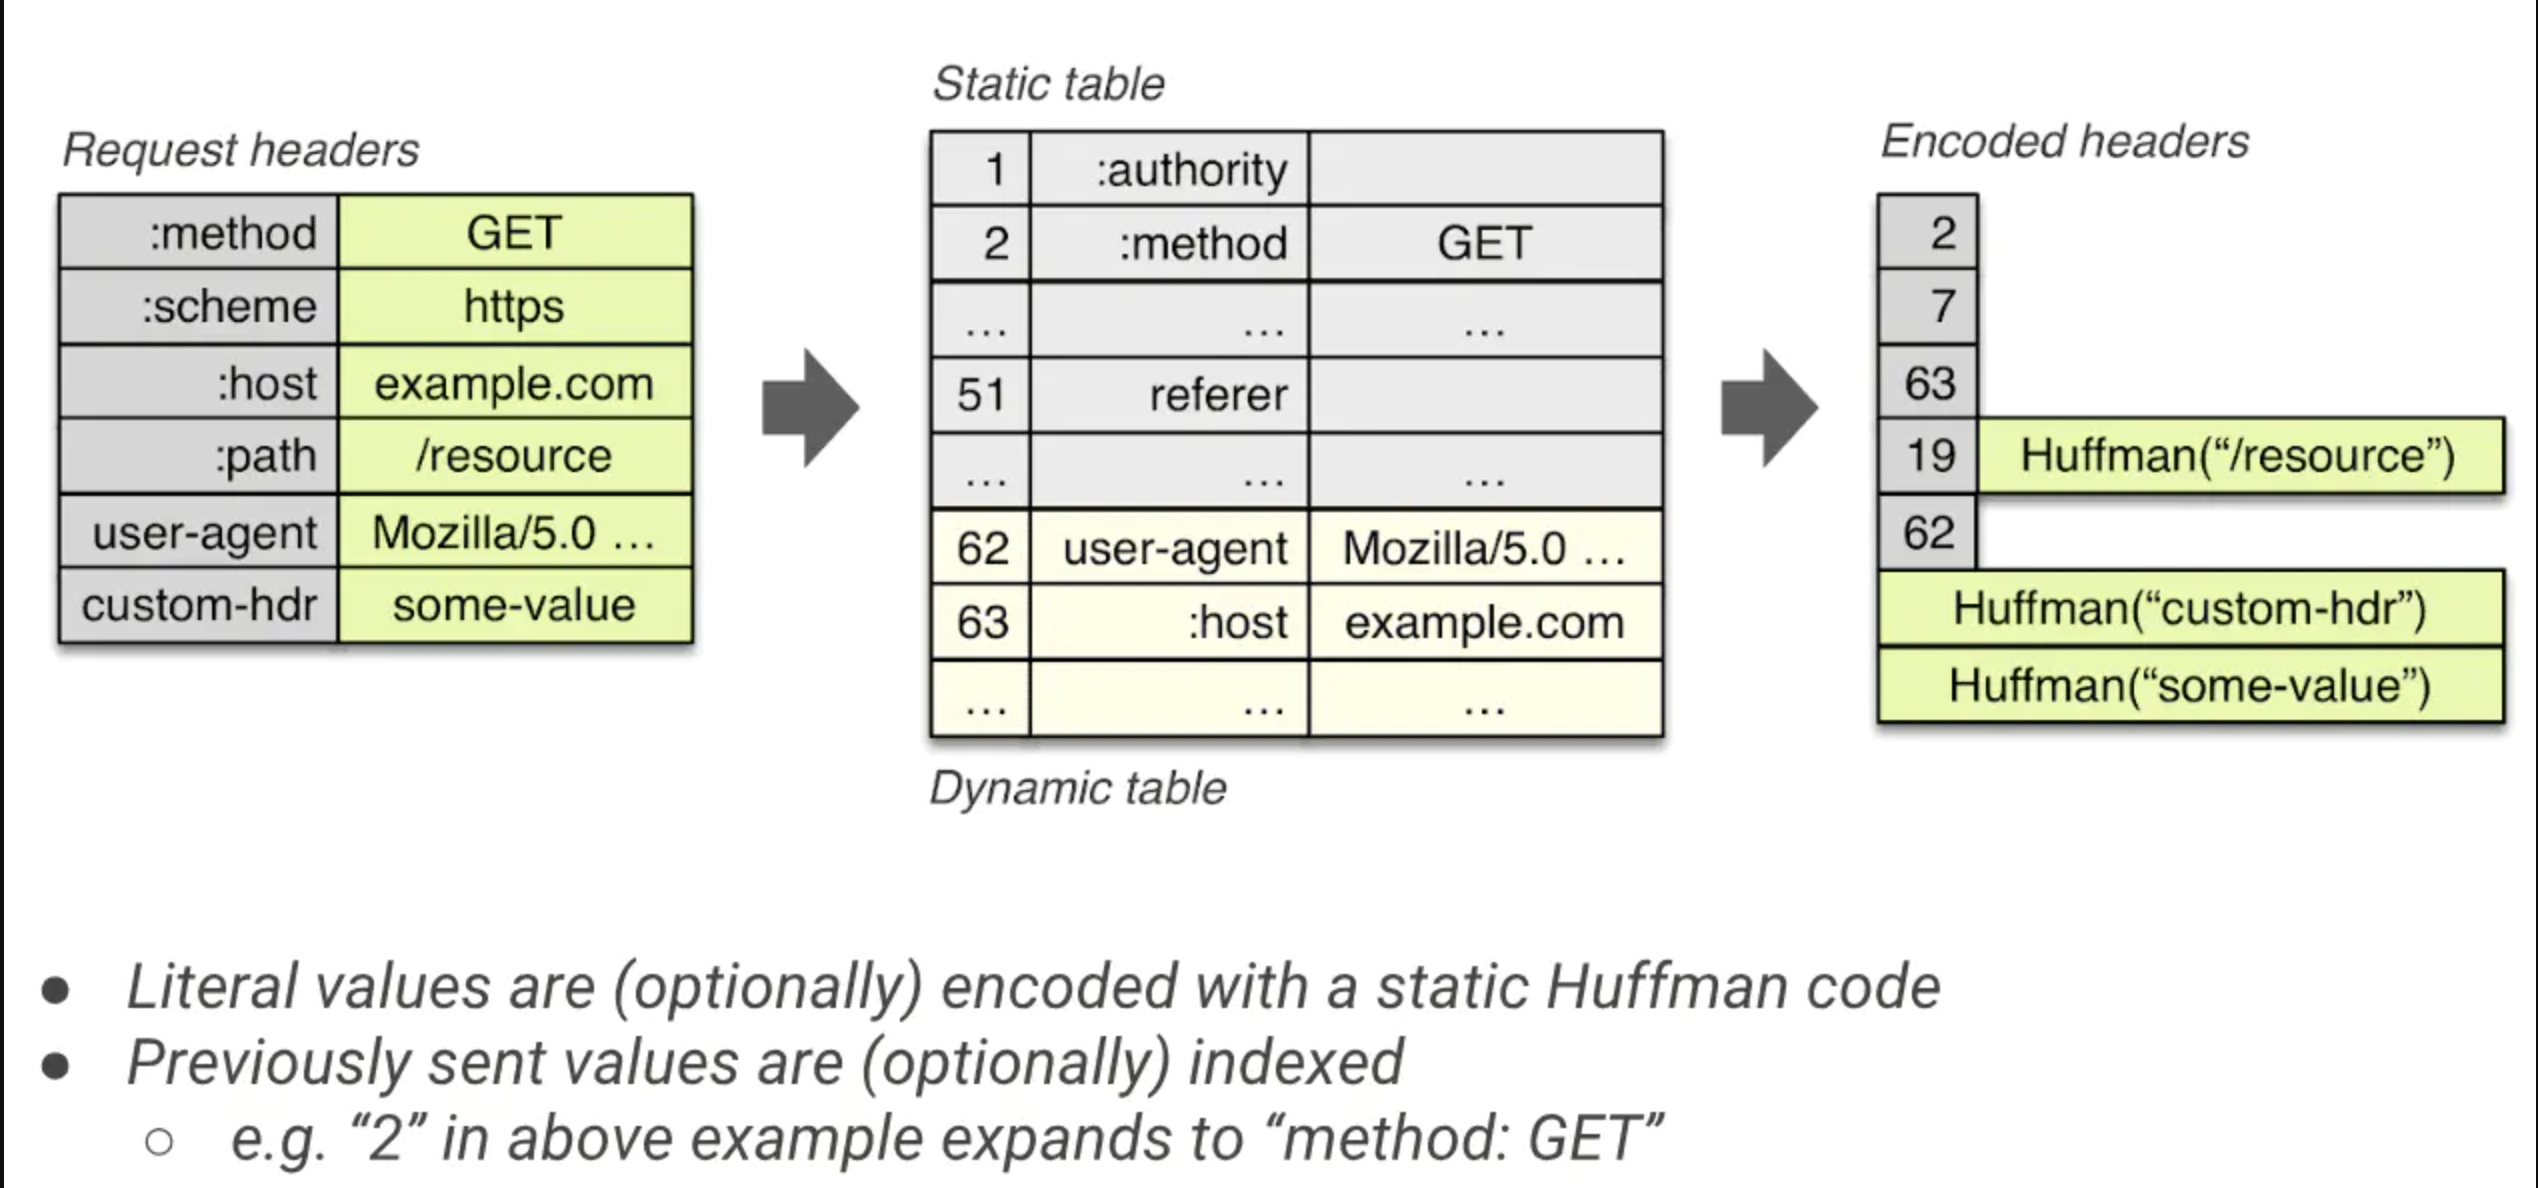
\includegraphics[width=1\textwidth]{http/http_2_hpack_get.png}
    \caption{Header压缩示例}
\end{figure}

......

\section{参考}

\href{https://tools.ietf.org/html/rfc7540}{Hypertext Transfer Protocol Version 2 (HTTP/2)} 

\href{https://tools.ietf.org/html/rfc7541}{HPACK: Header Compression for HTTP/2} 

\href{https://nghttp2.org/}{nghttp2}

\href{https://http2.golang.org/}{http2.golang}

\href{https://github.com/FiloSottile/mkcert}{mkcert}

\href{https://www.freecodecamp.org/news/how-to-get-https-working-on-your-local-development-environment-in-5-minutes-7af615770eec/}{How to get HTTPS working on your local development environment}

\href{https://http2.github.io/}{http2-spec}


《web性能权威指南》















































article, report, book und letter standard font size 

\begin{table}[]
    \begin{tabular}{|l|l|l|l|}
    \hline
                                    & \multicolumn{3}{l|}{standard font size} \\ \hline
    command                         &  10pt        & 11pt       & 12pt        \\ \hline
    \textbackslash{}tiny            &  5pt         & 6pt        & 6pt         \\ \hline
    \textbackslash{}scriptsize      &  7pt        &	 8pt	    & 8pt         \\ \hline
    \textbackslash{}footnotesize    &  8pt        &	 9pt	    & 10pt        \\ \hline
    \textbackslash{}small           &  9pt        &	 10pt       & 11pt        \\ \hline
    \textbackslash{}normalsize     &   10pt       &	 11pt       & 12pt        \\ \hline
    \textbackslash{}large          &   12pt       &	 12pt       & 14pt        \\ \hline
    \textbackslash{}Large          &   14pt       &	 14pt       & 17pt        \\ \hline
    \textbackslash{}LARGE    	   &   17pt       &	 17pt       & 20pt        \\ \hline
    \textbackslash{}huge           &   20pt       &	 20pt       & 25pt        \\ \hline
    \textbackslash{}Huge           &   25pt       &	 25pt       & 25pt        \\ \hline
    \end{tabular}
    \end{table}




%\\newpage 分页命令


%\\par:分段

\end{document}                                                            % The required last line
